\documentclass[14pt]{extreport}
\usepackage{gost}
\usepackage{listings}
\usepackage{fancyvrb}

%Тут можно вставить дополнительные пакеты

\begin{document}
	\lstset{ %
		language=Python,                % Язык программирования 
		numbers=left,                   % С какой стороны нумеровать
		basicstyle=\scriptsize,
		inputencoding=utf8,
		extendedchars=\true
	}
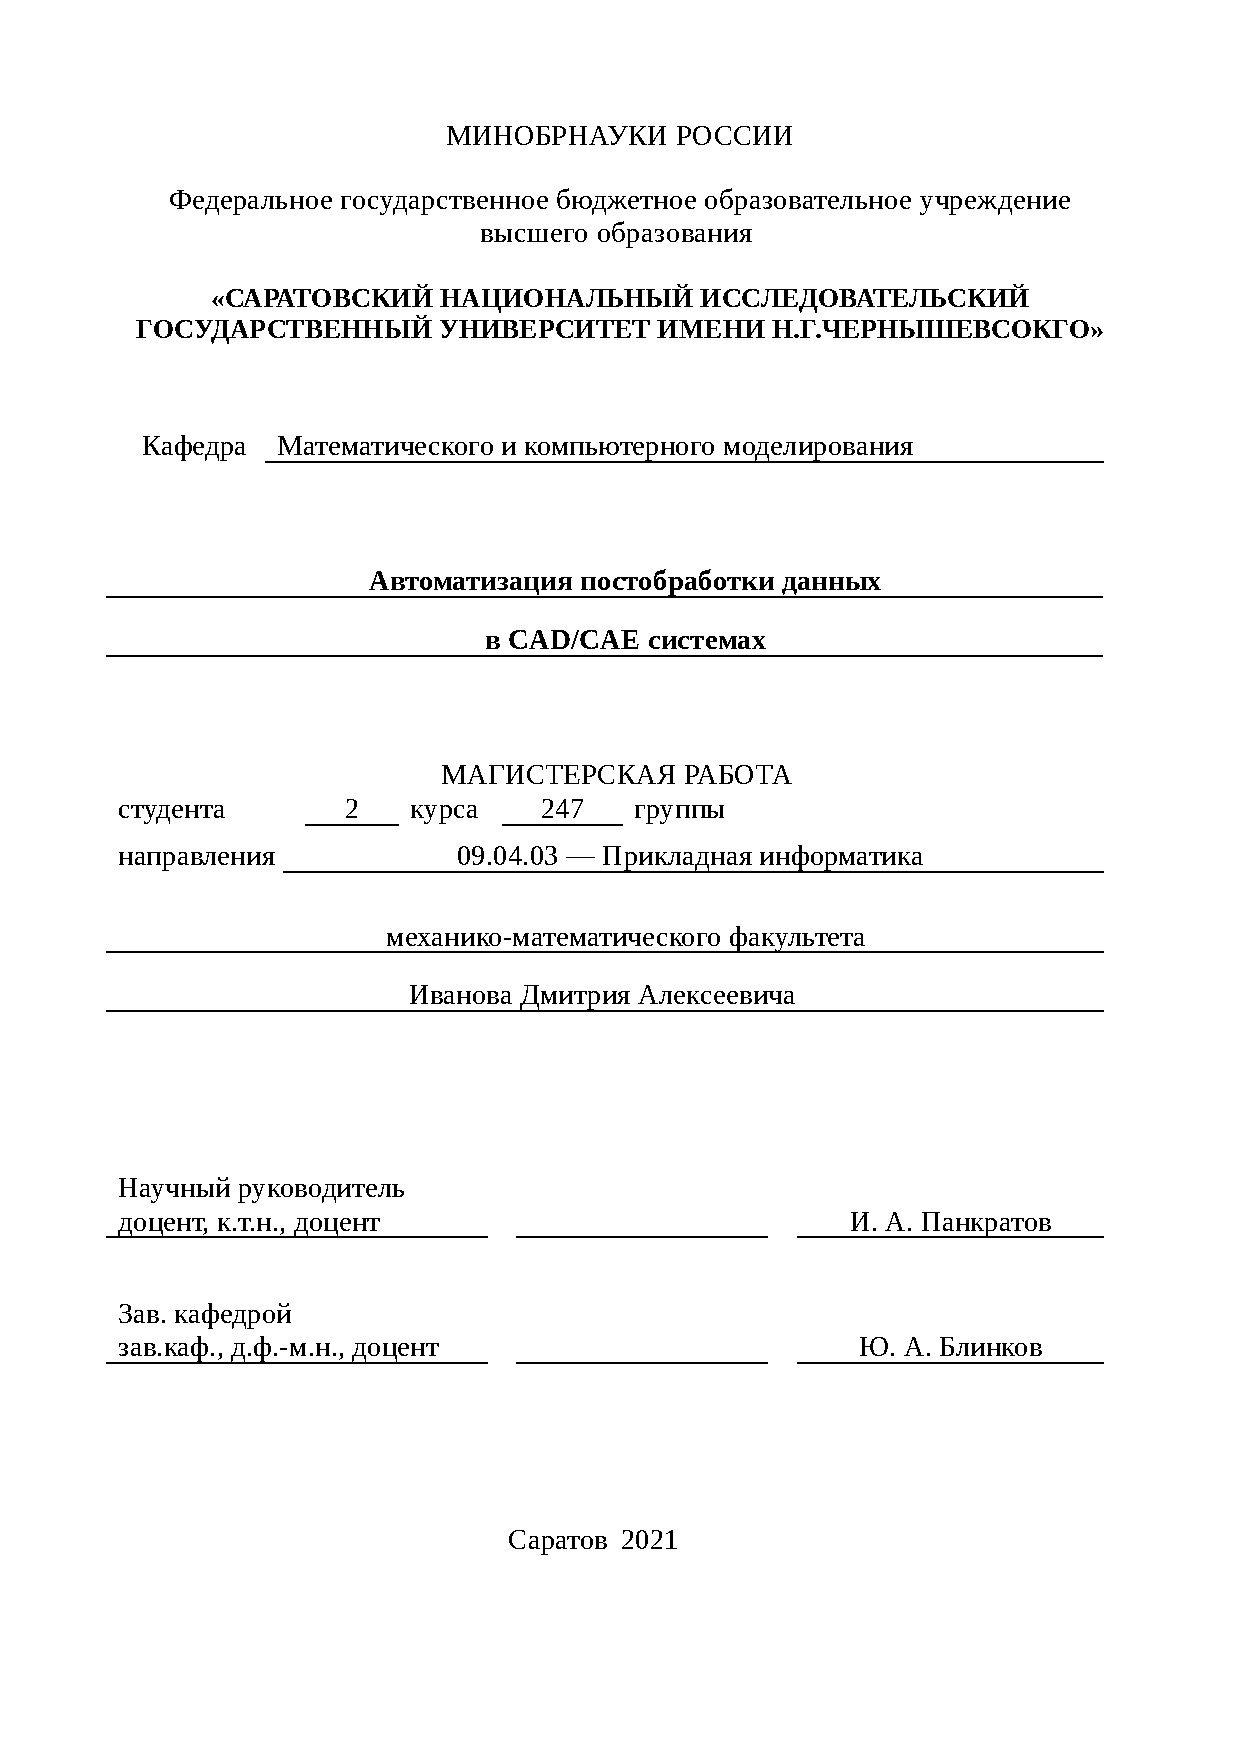
\includepdf[pages={1}]{titulCourse.pdf}

% ТЕМА: Анализ экспериментальных данных с помощью NoSQL

\tableofcontents

\abbreviations

CAD (от англ. Computer-aided design) -- автоматизированная система, реализующая информационную технологию выполнения функций проектирования;

CAE (от англ. Computer-aided engineering) -- общее название для программ и программных пакетов, предназначенных для решения различных инженерных задач;

CFD (от англ. Сomputational fluid dynamics) -- вычислительная гидродинамика;

БД -- база данных;

СУБД -- система управления базами данных;

виджет -- примитив графического интерфейса пользователя;

ИС -- информационная система. 

\intro

При обработке экспериментальных данных и расчетов, полученных в результате математического моделирования физических процессов в CAD/CAE системах, особенно, когда проводится, например, серия экспериментов, в которых входные данные незначительно изменяются часто порождается большой объем результатов, подлежащих анализу или иными словами -- постобработке. Причем, зачастую для анализа необходимо провести однотипные манипуляции с полученными мало различающимися данным. Учитывая все вышесказанное, становится ясна необходимость автоматизации такого процесса постобработки данных. 

В магистерской работе была спроектирована и разработана ИС позволяющая упростить процесс анализа полученных экспериментальных данных. Для автоматизации был использован язык программирования Python, для хранения результатов -- NoSQL подход, а конкретно СУБД MongoDB. 

Таким образом целью данной магистерской работы является проектирование и разработка информационной системы, автоматизирующей рутинные операции анализа экспериментальных данных.
Задачи:
\begin{itemize}
\item Кратко рассмотреть платформу для численного моделирования OpenFOAM и пакет для визуализации ParaView.
\item Рассмотреть существующие решения по данной тематике.
\item Спроектировать информационную систему и создать UML-диаграммы для ее описания.
\item Провести обзор средств разработки.
\item Разработать помогающую в анализе экспериментальных данных информационную систему.
\end{itemize}

\chapter{Об OpenFOAM и ParaView}
\section{OpenFOAM}
OpenFOAM (англ. Open Source Field Operation And Manipulation CFD ToolBox) — открытая интегрируемая платформа для численного моделирования задач механики сплошных сред ~\cite{OpenfoamWiki}.

Это пакет программ распространяемых свободно под лицензией GNU GPL, позволяющей решать задачи механики сплошных сред, в частности: 
\begin{itemize}
\item Прочностные расчеты;
\item Гидродинамика ньютоновских и неньютоновских вязких жидкостей как в несжимаемом, \item так и сжимаемом приближении с учётом конвективного теплообмена и действием сил гравитации. Для моделирования турбулентных течений возможно использование RANS-моделей, LES- и DNS-методов. Возможно решение дозвуковых, околозвуковых и сверхзвуковых задач;
Задачи теплопроводности в твёрдом теле;
\item Многофазные задачи, в том числе с описанием химических реакций компонент потока;
\item Задачи, связанные с деформацией расчётной сетки;
\item Сопряжённые задачи;
\item Некоторые другие задачи, при математической постановке которых требуется решение дифференциальных уравнений в частных производных в условиях сложной геометрии среды;
\end{itemize}

В основе кода лежит набор библиотек, предоставляющих инструменты для решения систем дифференциальных уравнений в частных производных как в пространстве, так и во времени. Рабочим языком кода является C++. OpenFOAM состоит из приблизительно 250 программ основанных на более чем 100 библиотеках. Каждое приложения выполняет свою конкретную задачу в рамках процесса расчета. Этапы работы представленные в соответствии с рисунком ~\ref{fig1}.

\begin{figure}[H]
\centerline{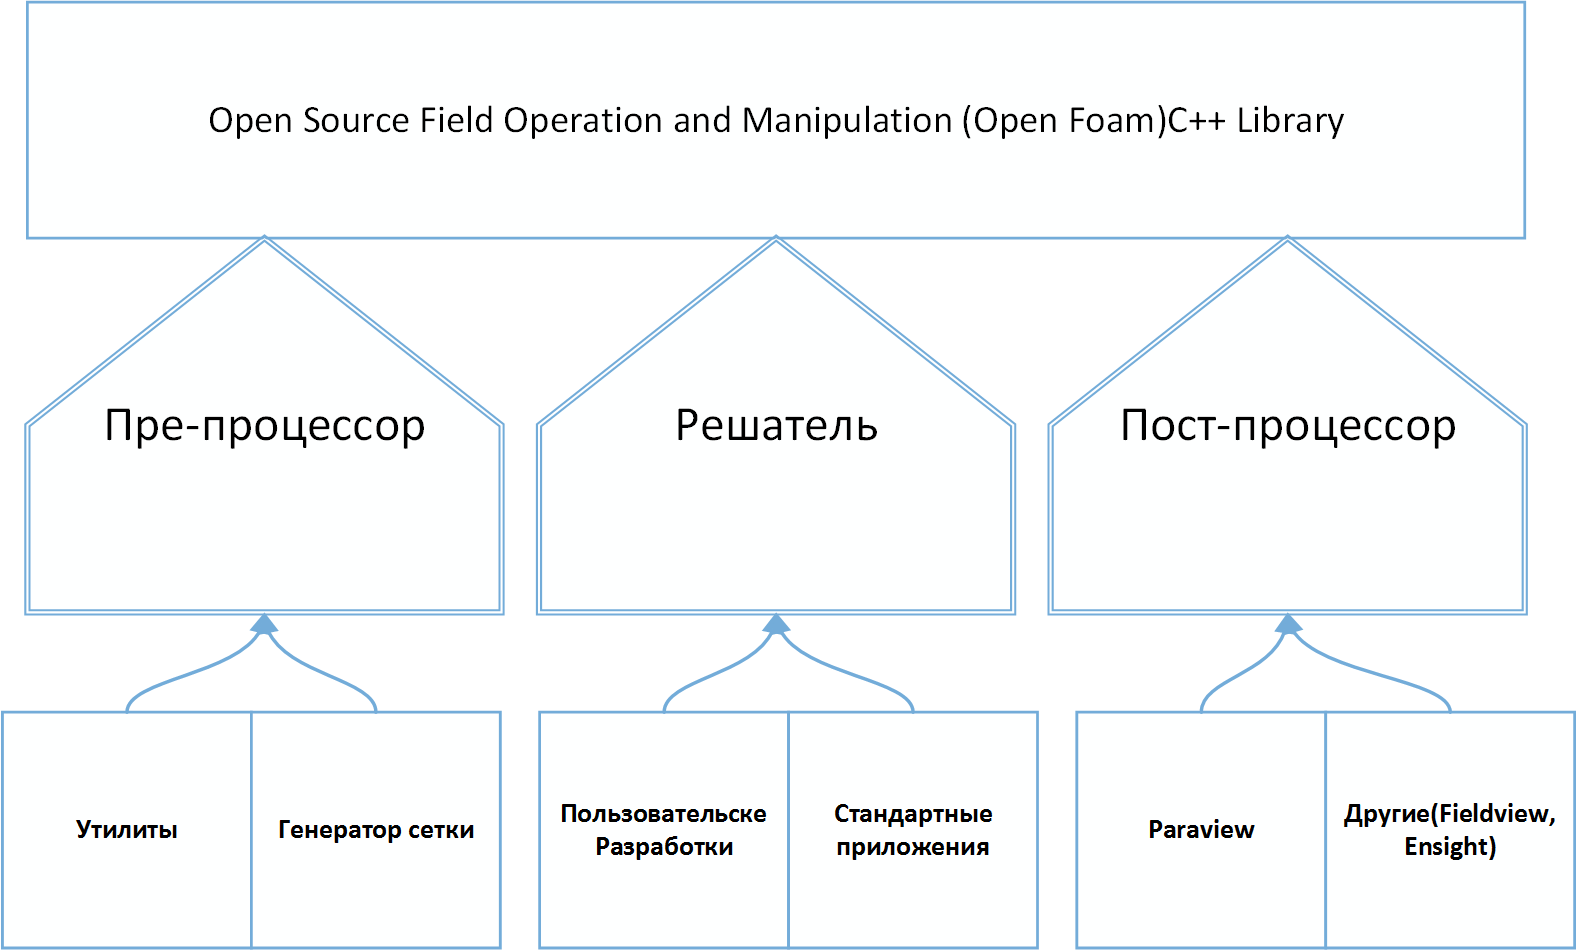
\includegraphics[width=1.0\linewidth]{OFScheme}}
\caption{Утилиты и программы входящие в пакет OpenFOAM, сгруппированные по этапам работы с расчетом}
\label{fig1}
\end{figure}

Работа с программой делится на три этапа:
\begin{enumerate}
\item Препроцессинг;
\item Решение;
\item Постпроцессинг.
\end{enumerate}

На этапе препроцессинга в специальных файлах задаются входные данные для рассчета примера, такие как: начальное время, конечное, шаг и так далее. Также параметры для хранения решения: время, формат, тип сжатия. Также в препроцессинг включены настройки выбора различных схем расчета, которые влияют на точность и стабильность решения. После этого отдельно генерируется расчетная область (сетка), которая впоследствии может быть обработана различными утилитами ~\cite{OpenfoamUserGuide}. Затем запускается решатель, который производит расчет. На этапе постпроцессинга полученные данные представляются в виде графиков. Также используются некоторые утилиты, например для конвертации из внутреннего формата OpenFOAM в широко используемый формат vtk.

\section{ParaView}
ParaView -- открытый графический кросс-платформенный пакет для интерактивной визуализации в исследовательских целях, разрабатываемый Национальной Лабораторией Сандиа, компанией Kitware и Национальной Лабораторией Лос-Аламоса \cite{ParaviewAbout}.

Пакет ParaView предоставляет пользователю возможности интерактивной визуализации и исследования больших массивов данных для качественного и количественного анализа.

Пакет может быть использован на компьютерах с операционными системами Windows, Linux, Mac OS X.

При разработке авторы придерживаются следующих целей:
\begin{itemize}
\item Открытость, кросс-платформенность — в пакете используются только открытые, мульти-платформенные технологии для визуализации данных.
\item Поддержка различных, в том числе, гетерогенных вычислительных систем.
\item Создание гибкого, интуитивного пользовательского интерфейса.
\end{itemize}

Таким образом, пакет ParaView во многом является скорее технологией обработки, чем всего лишь программным средством ~\cite{ParaviewWiki}.

Некоторые возможности пакета:
\begin{itemize}
\item Визуализация расчетных областей.
\item Визуализация полей (давление, скорость, температура, смещения и прочее).
\item Построение срезов областей как плоскостью, так и заданной функцией.
\item Построение изо-поверхностей.
\item Построение векторных полей и линий тока.
\item Позволяет показывать динамику развития протекающего процесса, отображая анимацию. 
\end{itemize}

Основной формат данных ParaView -- VTK, но пакет также содержит драйверы для работы с форматом OpenFOAM и поставляется вместе с дистрибутивом пакета. 

Работа с ParaView может осуществляться как в интерактивном, так и пакетном режиме.

ParaView также предлагает богатый и мощный програмный интерфейс на языке Python. Это позволяет пользователям автоматизировать обработку своих данных и использовать возможности, так называемого, набора инструментов визуализации -- Visualization Tool Kit (VTK) ~\cite{ParaviewAndPython}.

\chapter{Обзор существующих решений}
Информационная система должна выполнять постобработку данных, полученных в результате численно эксперимента в пакете OpenFOAM, делая упор на автоматизацию функций для работы с серией данных. Рассмотрим доступные приложения осуществляющие автоматизацию рутинных функций в рамках пакета OpenFOAM.
\section{HELYX OS}
HELYX-OS - это графический пользовательский интерфейс с открытым исходным кодом, разработанный компанией ENGYS для работы со стандартными библиотеками OpenFOAM, предоставляемыми OpenFOAM Foundation и ESI-OpenCFD. Приложение предназначено для академического использования и работы с CFD начального уровня. Распространяется в соответствии с GNU General Public License ~\cite{Helyx}.

HELYX-OS предоставляет полностью интерактивную, простую в использовании среду для выполнения всех задач предварительной обработки в процессе CFD, включая создание сетки, определение случая и выполнение решателя.

Существует также версия для корпоративного использования -- CFD HELYX.

Преимущества: 
\begin{itemize}
\item Встроенная поддержка как OpenFOAM, так и OpenFOAM+: возможность загружать существующие примеры, читая настройки непосредственно из доступных текстовых файлов проекта.
\item Программа доступна на платформах Linux и Windows. Однако версия для Windows платна.
\item Управление утилитой построения сеток snappyHexMesh, включая такие возможности как отображение геометрии и непосредственное построение прямо в окне приложения.
\item Отдельный мониторинг решателя с отслеживанием остатков решения.
\end{itemize}

В корпоративной версии также следует выделить:
\begin{itemize}
\item Высокая масштабируемость.
\item Возможность работы с использованием облачных технологий.
\item Модульность. Возможно расширение в рамках HELYX ADD-ONS, 
\end{itemize}

В соответствии с рисунком ~\ref{fig2} изображен рабочий экран программы.

\begin{figure}[H]
\centerline{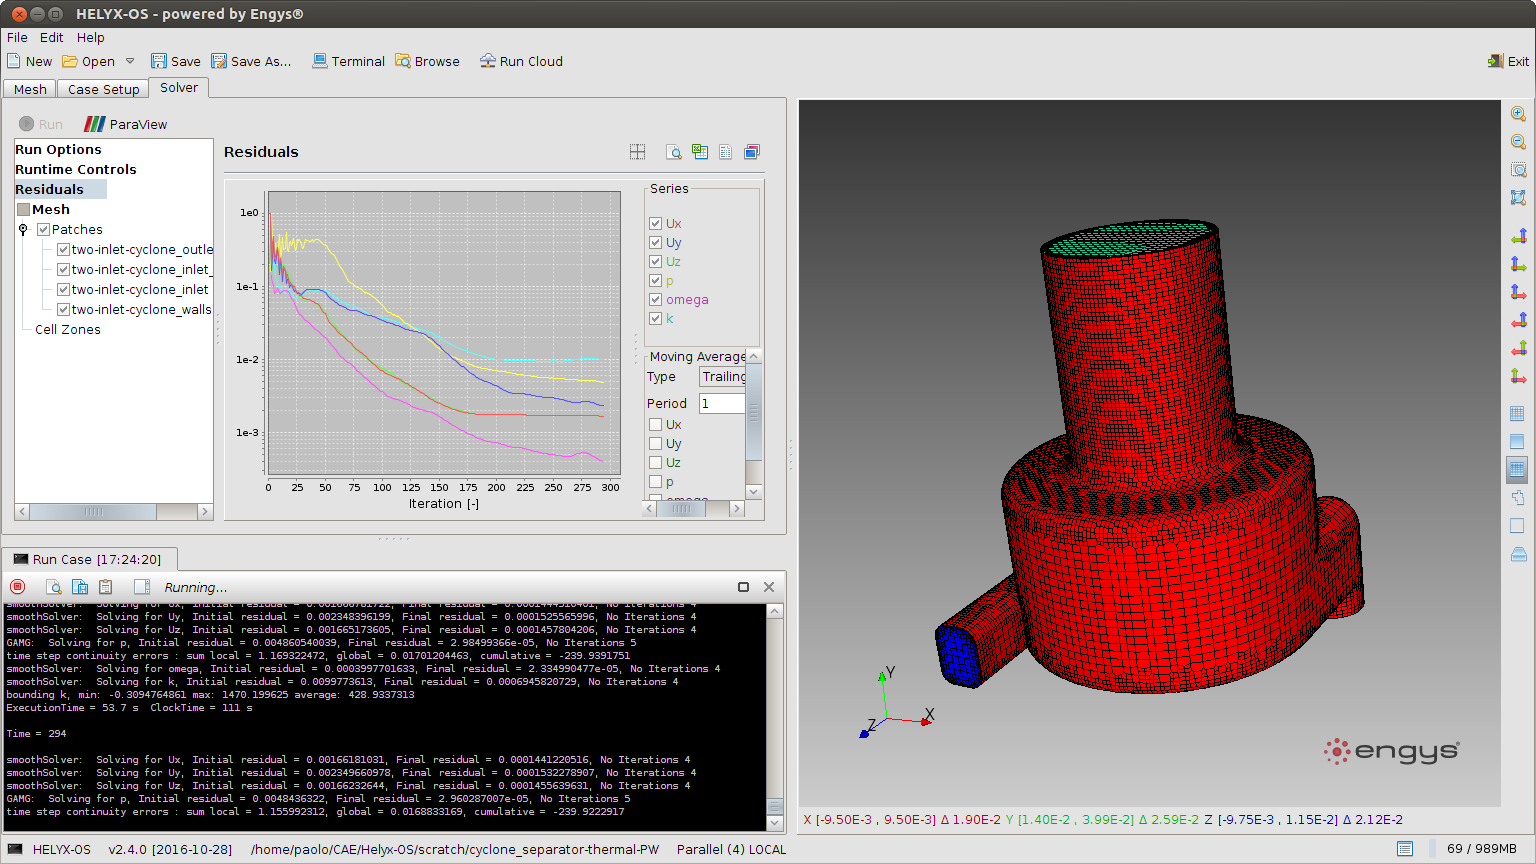
\includegraphics[width=1.0\linewidth]{helyxos}}
\caption{Рабочий экран приложения Helyx OS}
\label{fig2}
\end{figure}

\section{ANSA}
ANSA - это инструмент препроцессинга CAE, который предоставляет все необходимые функциональные возможности для построения полной модели, от CAD-данных  до готового к вводу файла решателя, в единой интегрированной среде ~\cite{Ansa}.

Все функции программного обеспечения размещены в интегрированной среде с настраиваемым графическим интерфейсом. Программное обеспечение доступно для всех современных популярных операционных систем в 32-битной и 64-битной архитектуре с использованием многоядерных процессоров. 

Преимущества: 
\begin{itemize}
\item Эффективная обработка данных для сложных структур моделей.
\item Быстрое и качественное моделирование сложных геометрических моделей.
\item Возможность взаимодействия между моделями, созданными для разных решателей.
\item Высокоавтоматизированные процессы и инструменты настройки модели в одной программе.
\item Уменьшены зависящие от пользователя подверженные ошибкам операции.
\item Полное построение модели для многочисленных решателей в одной среде.
\end{itemize}
Рабочий экран приложения представлен в соответствии с рисунком ~\ref{fig3}.

\begin{figure}[H]
\centerline{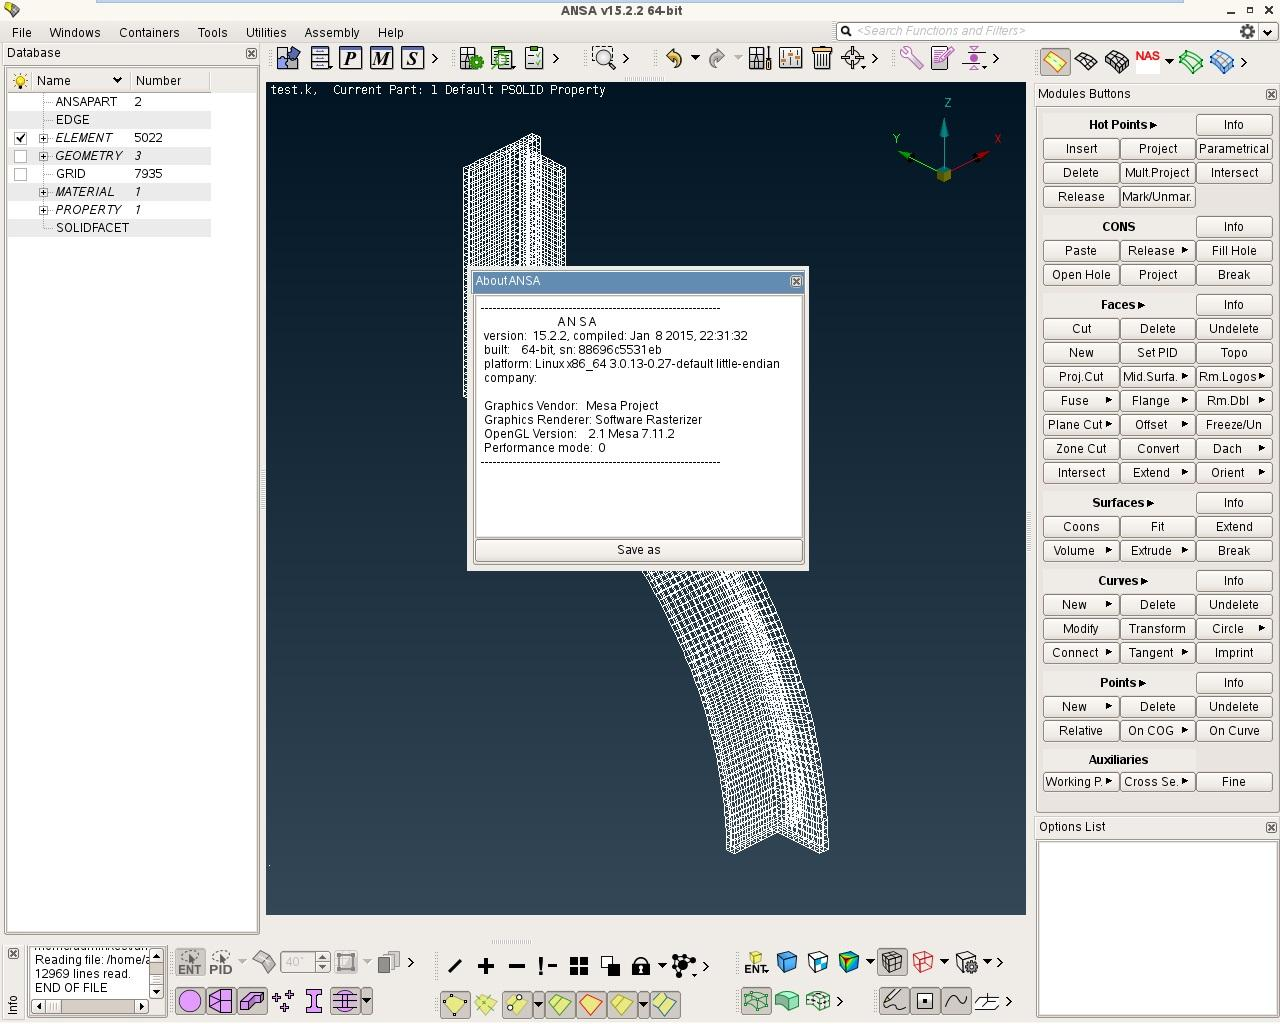
\includegraphics[width=1.0\linewidth]{ansa}}
\caption{Рабочий экран приложения ANSA}
\label{fig3}
\end{figure}

\section{CastNet}

CastNet упрощает использование технологических решений CAE для решателей с открытым исходным кодом: кроме типичного редактирования текстовых файлов, предоставляется альтернативный способ работы с OpenFOAM на основе графического интерфейса, сохраняя полную совместимость со стандартными выпусками OpenFOAM. В результате рабочий процесс становится достаточно гибким, и пользователь может в любой момент переключаться между настройкой рабочего примера на основе текстового файла и графического интерфейса пользователя.

Вид рабочего экрана приложения представлен в соответствии с рисунком ~\ref{fig4}
\begin{figure}[H]
\centerline{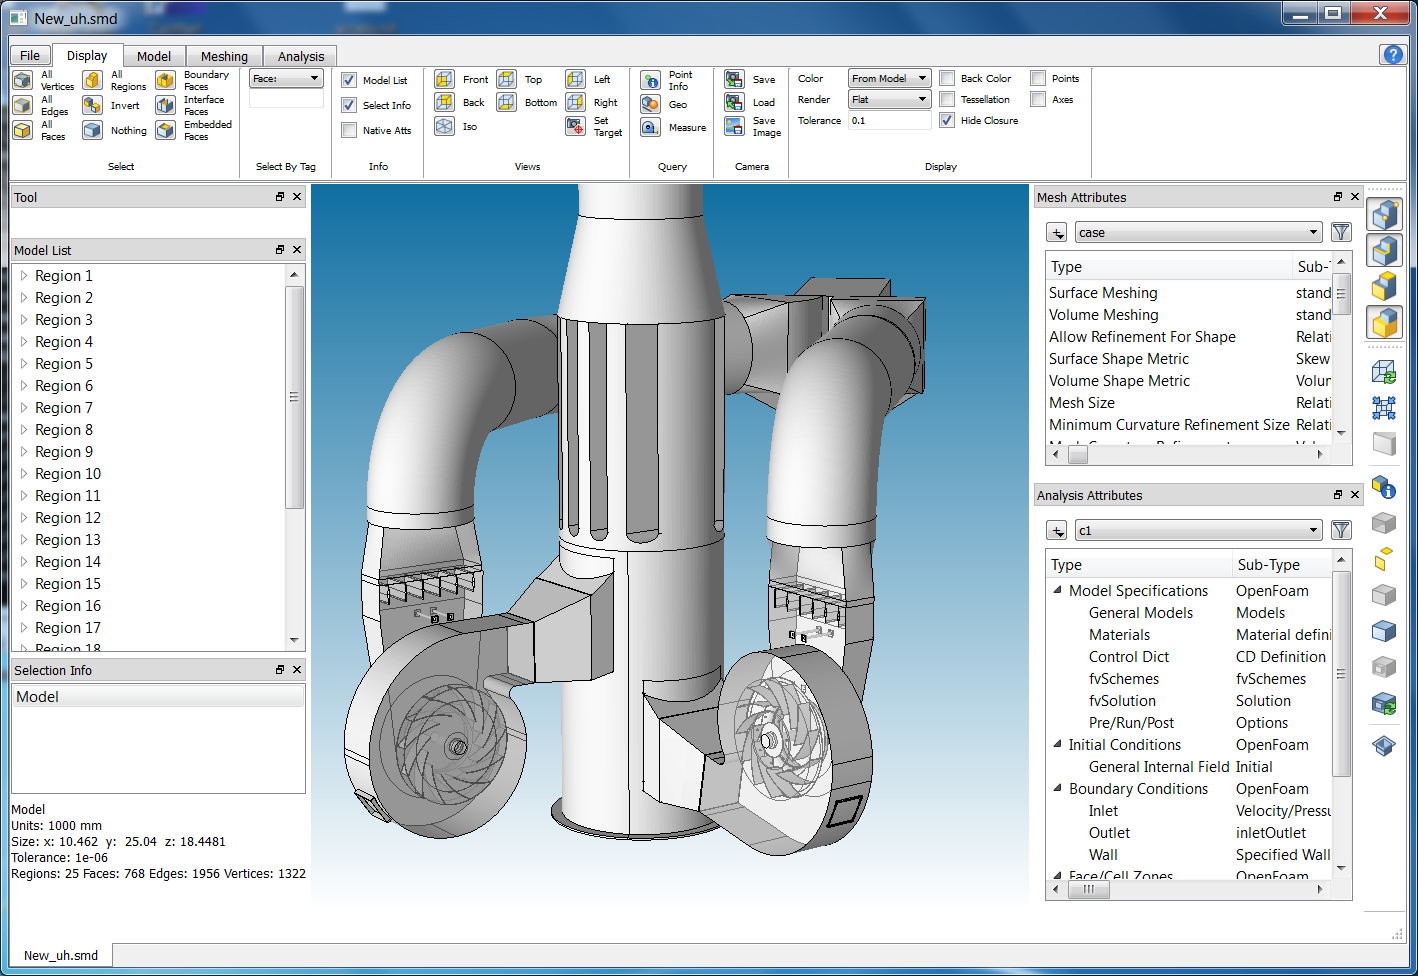
\includegraphics[width=1.0\linewidth]{castnet}}
\caption{Рабочий экран приложения CastNet}
\label{fig4}
\end{figure}

Ключевые особенности CastNet:
\begin{itemize}
\item Среда разработки на основе графического интерфейса пользователя, включающая предварительную обработку (создание сетки, настройку примера), мониторинг решения и последующую обработку. Таким образом: доступ к мощным функциям решателя с открытым исходным кодом без редактирования текстовых файлов или необходимости детального изучения структуры ключевых слов OpenFOAM.
\item Кроссплатформенное использование: поддержка среды для пакета программ OpenFOAM в операционных системах Windows и Linux.
\item Библиотека шаблонов позволяет настраивать пример для более чем 30 решателей.
\item Больше надежности в отношении результатов моделирования благодаря контролю сходимости.
\end{itemize}

\section{Выводы}

Таким образом, рассмотренные существующие решения предлагают разнообразные и гибкие возможности по работе с примерами:
\begin{itemize}
\item CastNet интегрирована с OpenFoam, имеет графический интерфейс, но работает только одним конкретным примером. \item Ansa -- мощный инструмент препроцессинга. Имеет высокоавтоматизированные процессы и инструменты настройки модели в одной программе. Возможность быстро и качественно моделировать сложных геометрических модели, но ничего не сказано о какой-либо работе с группой моделей. 
\item HELYX-OS имеет встроенную поддержку OpenFOAM, предоставляет возможности отображения геометрии и непосредственного построения примера прямо в окне, но также не концентрируется на работе с набором примеров. 

Однако, ни одно из них не предоставляет функциональности по работе сразу с группой примеров, что в свою очередь вызывает трудности при анализе экспериментальных данных, которые состоят из набора примеров.  
\end{itemize}

\chapter{Проектирование информационной системы}
\section{Постановка задачи}
Необходимо спроектировать приложение, которое бы выполняло процесс постобработки, то есть строило графики, используя экспериментальные данные, полученные из пакета программ OpenFOAM. Приложение должно также работать с группами экспериментальных данных, то есть выполнять конкретное действие построения графика, например срез, с группой из разных мало отличающихся примеров. Программа должна хранить экспериментальные данные и историю операций примера, также должна быть реализована возможность экспорта графиков в файлы.
Для более подробного понимания информационной системы были построены UML-диаграммы. 

\section{Диаграмма прецедентов}
Прецеденты -- это технология определения функциональных требований к системе ~\cite{umlDistilled}. 
Диаграмма прецедентов (use case diagram) предназначена для описания взаимодействия проектируемой системы с любыми внешними или внутренними объектами - пользователями, другими системами и тому подобное.
Основными понятиями при работе с диаграммой вариантов использования являются 
Актор (Actor) -- это роль, которую выполняет пользователь или другая система, при взаимодействии с проектируемой системой.
Вариант использования -- это конечная единица взаимодействия актора и системы. 

Диаграмма вариантов использования представлена в соответствии с рисунком ~\ref{fig5}
\begin{figure}[H]
\centerline{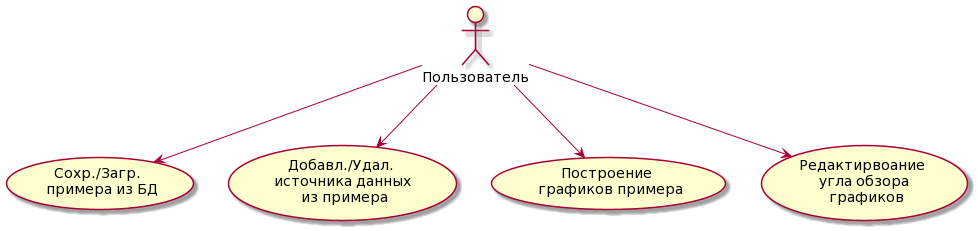
\includegraphics[width=1.0\linewidth]{userCaseDiagram}}
\caption{Диаграмма прецедентов}
\label{fig5}
\end{figure}

Ниже представлен код генерации диаграммы прецедентов при помощи инструмента PlantUML.
\begin{Verbatim}[numbers=left,xleftmargin=5mm,fontsize=\small]
@startuml
actor "Пользователь" as user
user-->(Сохр./Загр. \n примера из БД)
user-->(Добавл./Удал. \n источника данных \n из примера)
user-->(Построение \n графиков примера)
user-->(Редактирвоание \n угла обзора \n графиков)
@enduml
\end{Verbatim}

В соответствии с рисунком ~\ref{fig5} представлена базовая функциональность проектируемой программы. Пример или основная сущность программы состоит из списка источников данных. Каждый источник данных -- это результат конкретного численного эксперимента. Таким образом достигается цель -- работа сразу с несколькими источниками данных.   

В случае описанной программы, встречаются следующие прецеденты:
\begin{itemize}
	\item Сохранение и загрузка примера из базы данных. Работа с программой строится вокруг анализа расчетов полученных от пакета программ OpenFOAM, конфигурации данных должны сохраняться в БД для обеспечения сохранности информации и быстрого доступа к ней, при возрастающим объеме примеров. 
	\item Добавление и удаление источника данных из примера. Также необходимая функция для возможности быстрой и гибкой настройки примеров для получения различных срезов и углов обзора графиков.
	\item Редактирование угла обзора графиков -- изменение положения камеры в соответствии с необходимостью анализа данных.
	\item Построение графиков примера -- получение изображение в соответствии с описанными выше настройками примера.
\end{itemize}

\section{Диаграмма классов}
Диаграмма классов описывает типы объектов системы и различного рода статические отношения, которые существуют между ними. На диаграммах классов отображаются также свойства классов, операции классов и ограничения, которые накладываются на связи между объектами ~\cite{umlDistilled}.

Для удобства рассмотрения разобьем диаграмму классов на три рисунка. Каждый из которых соответствует определенной решаемой задачи. 

\subsection{Диаграмма модели данных}
В соответствии с рисунком ~\ref{fig6} представленная диаграмма классов,
иллюстрирует способ организации модели данных хранящих кейс для генерации данных. Кейс или пример -- основная сущность программы. В ней хранится текущее частичное состояние. Модель состоит из набора связанных сущностей, модели хранятся в списке -- который описывает полное состояние системы.



\subsection{Диаграмма, представляющая способ организации экспериментальных данных}

В соответствии с рисунком \ref{fig6} представленная диаграмма классов иллюстрирует способ организации экспериментальных данных в приложении. 

В соответствии с рисунком \ref{fig6} основным классом модели является FoamCase. В нем хранится все необходимое для генерации различных графиков. Соответственно его поля -- это параметры генерации:
\begin{itemize}
	\item CasesDir -- класс, который хранит путь к примеру. Пример это директория, содержащая один или несколько кейсов OpenFOAM.
	
	Код для генерации класса CaseDir:	
	\begin{Verbatim}[numbers=left,xleftmargin=5mm,fontsize=\small]
	class CasesDir{
		+idn: int
		+path: Path
	}
	\end{Verbatim}
	
	\item CameraProps -- класс, который содержит настройки камеры для построения графика.
	
	\begin{Verbatim}[numbers=left,xleftmargin=5mm,fontsize=\small]
	class CameraProps{
		+idn: int
		+name: str
		+focal_point: Point
		+cam_position: Point
		+viewup: Point
		+viewangle: float
	}
	\end{Verbatim}
	\item Point -- утилитарный класс, необходимый для представления данных с точки зрения позиции камеры для обзора.
	
	\begin{Verbatim}[numbers=left,xleftmargin=5mm,fontsize=\small]
	class Point{
		+x: float
		+y: float
		+z: float
	}
	\end{Verbatim}
	\item SharedState -- Класс хранящий общую информацию для контролера и представления. Необходим пересылки общей универсальной информации высокого уровня между виджетами разных уровней отображения.
	
	В этом классе отдельно выделено важное поле case\_list -- оно хранит все текущие <<живые>>, иными словами доступные в бд и не удаленные пользователем, экземпляры класса FoamCase.
		\begin{Verbatim}[numbers=left,xleftmargin=5mm,fontsize=\small]
		class FoamCase{
			+idn: int
			+name: str
			+cases_dir: CaseDir
			+cam_prop_list: List[CameraoProps]
		}
		class Controller {}
		hide Controller members
		class SharedState {
			+case_list: List[FoamCase]
			+state1
			+state2
			+ ...
		}		
		\end{Verbatim}
	
\end{itemize}

А теперь необходимо установить связи между классами диаграммы: 
\begin{Verbatim}[numbers=left,xleftmargin=5mm,fontsize=\small]
Controller -- FoamCase
SharedState --o Controller
Point -- CameraProps
FoamCase "*" --o "1" SharedState
CasesDir "1" --* "1" FoamCase
CameraProps "*" --* "1" FoamCase
\end{Verbatim}

\begin{figure}[H]
\centerline{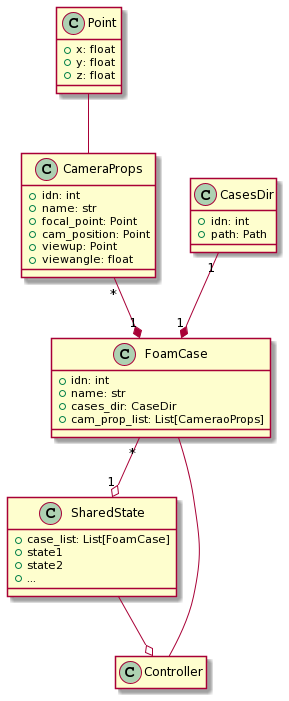
\includegraphics[height=1.0\linewidth]{model}}
\caption{Диаграмма классов, представляющая способ организации данных в приложении}
\label{fig6}
\end{figure}


\subsection{Диаграмма для работы с базой данных. Слой DAO}
В соответствии с рисунком ~\ref{fig7} представленная диаграмма классов, иллюстрирует структуру DAO слоя (Data Access Object). Этот слой необходим для получения различных сущностей из базы данных, абстрагируясь от того какая конкретно СУБД используется. 
Ход генерации данной диаграммы, как и разработку данных классов в приложении можно разбить на несколько этапов:
\begin{enumerate}[label=\Roman*.]
	\item Построение абстрактных классов фабрики классов DAO. Про паттерн фабрика будет подробнее сказано чуть ниже. Нужно отметить, что абстрактные классы, учитывая множественное наследование в Python выполняю и в некотором смысле роль интерфейсов.
	Ниже приведен код генерации абстрактного класса фабрики:
	\begin{Verbatim}[numbers=left,xleftmargin=5mm,fontsize=\small]
	abstract class DaoFactory{
		- DBConnection _get_connection()
		+ AbstractDAO get_dao(connection, dao_class)
	}
	\end{Verbatim}
	\item Следующий этап -- это расширение абстракции до конкретной фабрики DAO компонентов БД MongoDB:
	\begin{Verbatim}[numbers=left,xleftmargin=5mm,fontsize=\small]
	class MongoDaoFactory {
		- LOGIN
		- PASSWORD
		- MongoDBConnection MongoDBConnection _get_connection()
		+ MongoAbstractDAO MongoDget_dao(connection, dao_class)
	}
	\end{Verbatim}
	
	\item На этом этапе строиться абстрактные класс для DAO компоненты (выступает и в качестве интерфейса). Но также и абстрактный класс для MongoDB, созданный для того, чтобы избежать дублирования кода в при написании программы. Код генерации представлен ниже:
	\begin{Verbatim}[numbers=left,xleftmargin=5mm,fontsize=\small]
	abstract class AbstractDAO{
		+connection
		+Any create(obj)
		+Any create_or_update(obj)
		+Any read(key)
		+Any update(obj)
		+Any delete(key)
		+List[Any] get_all()
	}
	
	abstract class MongoAbstractDAO{
		+Any delete(key): implemented
		+Any get_all(): implemented
	}
	\end{Verbatim}

	\item Далее идет генерация уже конкретных классов DAO базы данных MongoDB:
	\begin{Verbatim}[numbers=left,xleftmargin=5mm,fontsize=\small]
	class MongoFoamCaseDAO{}
	hide MongoFoamCaseDAO members
	
	class MongoCaseDirDAO{}
	hide MongoCaseDirDAO members
	
	class MongoCameraPropsDAO{}
	hide MongoCameraPropsDAO members
	\end{Verbatim}

	\item На последней этапе были сгенерированы классы из сторонних модулей, ассоциациированные с DAO. Код представлен ниже:
	
	\begin{Verbatim}[numbers=left,xleftmargin=5mm,fontsize=\small]
	class Config {}
	hide Config members
	
	
	class Controller {}
	hide Controller members
	
	DaoFactory <|-- MongoDaoFactory
	Config ..> MongoDaoFactory: inject LOGIN, PASSWORD
	Controller -- DaoFactory
	Controller -- AbstractDAO
	DaoFactory --> AbstractDAO
	AbstractDAO <|-- MongoAbstractDAO
	MongoAbstractDAO <|--MongoFoamCaseDAO
	MongoAbstractDAO <|--MongoCaseDirDAO
	MongoAbstractDAO <|--MongoCameraPropsDAO
	\end{Verbatim}
	
	
\end{enumerate}

При проектирование также необходимо предусмотреть неуказанный в диаграмме класс DTO (Data Transfer Object). Он используется как объект в котором хранятся данные модели сущности при передаче в БД или внешний сервис. Это необходимо для того, чтобы при изменении стороннего модуля или представления в базе данных локализовать изменения, которые необходимо внести в разрабатываемой программе, в одном модуле.

Также был разработан отдельный модуль modelmapper. В нем единственный класс Mapper отвечает за преобразования объектов модели в их DTO-аналог и наоборот. Таким образом при возникновении изменений на стороне необходимо будет изменить соответствующий DTO-класс, а также его метод в классе Mapper. 

Для установления соединения и работы с базой данных используется класс из PyMongo, не отраженный на диаграмме, также для доступа к базе данных используется класс Config, который передает логин, пароль и дополнительную специфичную для конкретного соединения информацию. Класс Config (как и предоставляющий соединение с базой данных класс из PyMongo) реализован при помощи шаблона проектирования синглтон (Singleton). Данный паттерн гарантирует, что у класса есть только один экземпляр, и предоставляет к нему глобальную точку доступа ~\cite{oop}. Такой подход дает позволяет только один раз при первом обращении произвести ресурсоемкую операцию установления соединения с базой данных или чтения config-файла, а после каждый раз при последующих обращениях возвращать уже созданный экземпляр класса. 

Так как имеется три класса DAO, а вообще, их может быть и больше, был реализован паттерн фабрика. Фабричный метод — это порождающий паттерн проектирования, который определяет общий интерфейс для создания объектов в суперклассе, позволяя подклассам изменять тип создаваемых объектов \cite{pattern-factory}.

\begin{figure}[H]
	\centerline{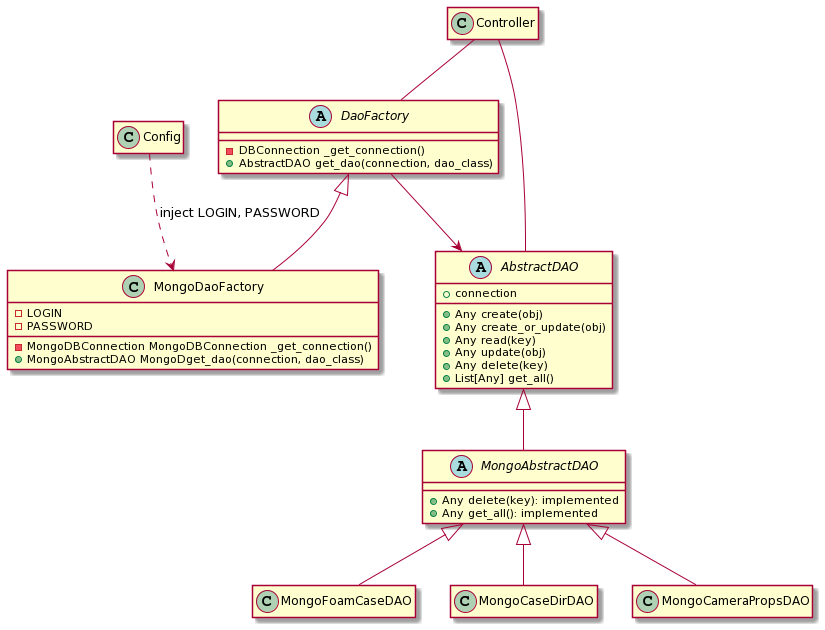
\includegraphics[width=1.0 \linewidth]{dao}}
	\caption{Диаграмма классов. Cлой DAO и его фабрика}
	\label{fig7}
\end{figure}


Использование этого шаблона дает следующие преимущества:
\begin{itemize}
\item Избавляет класс от привязки к конкретным классам продуктов.
\item Выделяет код производства продуктов в одно место, упрощая поддержку кода.
\item Упрощает добавление новых продуктов в программу.
\item Реализует принцип открытости/закрытости.
\end{itemize}

К недостаткам можно отнести возможность создания больших параллельных иерархий классов, так как для каждого класса продукта надо создать свой подкласс создателя.

Здесь же опишем подробнее класс Config. В нем, помимо одиночки, был реализован паттерн заместитель. 
Заместитель — это структурный паттерн проектирования, который позволяет подставлять вместо реальных объектов специальные объекты-заменители. Эти объекты перехватывают вызовы к оригинальному объекту, позволяя сделать что-то до или после передачи вызова оригиналу \cite{pattern-proxy}. 

При использовании библиотеки ConfigParser есть возможность для удобства пользователя разделять параметры по разделам. Поэтому удобно возвращать вместо конечных данных класс ConfigProxy, который в зависимости от раздела будет каким-то образом предобрабатывать данные. Например, приводить к нужному типу, или добавлять префикс к возвращаемому пути папки для сохранения данных. 

\subsection{Диаграмма классов для представлений (View)}

Здесь необходимо упомянуть что все классы кроме Controller наследуются от QWidget. И по своей сути это инструкции как собрать графический интерфейс пользователя. В дополнение к этому в этих классах происходит привязка функций обратного вызова (callback) контроллера к отображению через конструктор классов отображения. Этот факт отражен да диаграмме в виде ассоциаций. 


\begin{figure}[H]
	\centerline{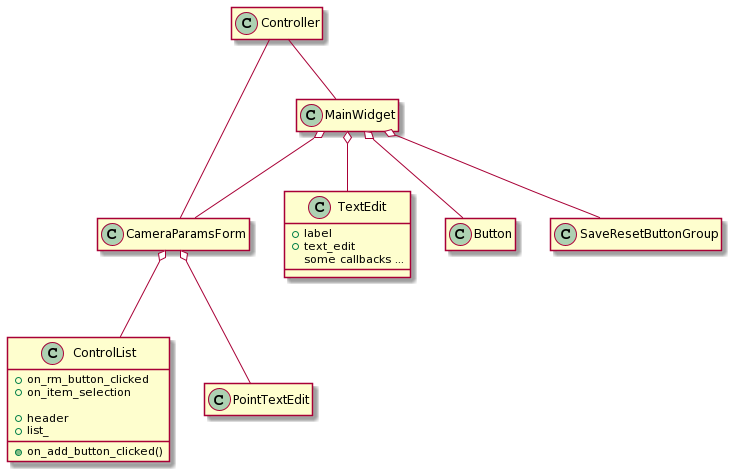
\includegraphics[width=0.8 \linewidth]{view}}
	\caption{Диаграмма классов. Отображение (View)}
	\label{fig8}
\end{figure}

В один из обработчиков событий кнопок <<на нажатие>> в Controller классе включен вызов метода takeScreenshot класса Screenshot. Этот метод обращается к Paraview API и генерирует график по заданным параметрам.

Далее приведен код генерации данной диаграммы: 
\begin{Verbatim}[numbers=left,xleftmargin=5mm,fontsize=\small]
@startuml
class ControlList {
	+on_add_button_clicked()
	+on_rm_button_clicked
	+on_item_selection
	+header
	+list_
class TextEdit {
	+ label
	+ text_edit
	some callbacks ...
}
class PointTextEdit{}
hide PointTextEdit members
class CameraParamsForm {}
hide CameraParamsForm members
class Button {}
hide Button members
class SaveResetButtonGroup {}
hide SaveResetButtonGroup members
class MainWidget {}
hide MainWidget members
class Controller {}
hide Controller members

MainWidget o-- SaveResetButtonGroup
MainWidget o-- Button
MainWidget o-- TextEdit
MainWidget o-- CameraParamsForm
CameraParamsForm o-- PointTextEdit
CameraParamsForm o-- ControlList
Controller -- MainWidget
Controller -- CameraParamsForm
@enduml
\end{Verbatim}


\section{Диаграмма последовательностей}
Диаграммы последовательностей или взаимодействия (interaction diagrams) описывают взаимодействие групп объектов в различных условиях их поведения. UML определяет диаграммы взаимодействия нескольких типов, из которых наиболее употребительными являются диаграммы последовательности (sequence diagram)~\cite{umlDistilled}.

На диаграмме последовательностей отображаются системные события для одного
сценария некоторого прецедента. Поэтому сама диаграмма строится на основе описания прецедента ~\cite{umlApplying}. 

Если прецедент отвечает на вопрос <<Что делает актор?>>, то последовательность отвечает на вопрос <<Как работает система при выполнении данного прецедента?>>.
Каждый прецедент может содержать несколько диаграмм последовательностей, на тот случай, если они описывают несколько альтернативных вариантов развития событий.

Диаграмма последовательностей будет построена только для прецедента <<Построение графиков примера>>, <<Сохранение примера в базу данных>>, <<Добавление источника 
данных>>. 

Ниже представлен код генерации диаграммы последовательностей для прецедента <<Построение графиков примера>>:
\begin{Verbatim}[numbers=left,xleftmargin=5mm,fontsize=\small]
@startuml
participant Пользователь

Пользователь -> ":Controller" : построить графики
create ":Screenshot"
activate ":Controller"
":Controller" -> ":Screenshot" : обратиться к классу
":Controller" -> ":Screenshot" : take_screenshot(cases_list, output)
activate ":Screenshot"
deactivate ":Controller"
":Screenshot" -> ":FoamCase" : get_data()
activate ":FoamCase"
":FoamCase" --> ":Screenshot" : вернуть data
deactivate ":FoamCase"
":Screenshot" -> ":ParaView" : set_data()
activate ":ParaView"
":Screenshot" -> ":ParaView" : show()
":ParaView" -> ":Screenshot" : вернуть графики
":Screenshot" -> ":ParaView": сохранить графики
deactivate ":Screenshot"
":ParaView" -> Пользователь: вернуть файлы с построенными графиками
deactivate ":ParaView"
@enduml
\end{Verbatim}

В соответствии с рисунком ~\ref{fig9} представлена диаграмма последовательностей для прецедента <<Построение графиков примера>>.

\begin{figure}[H]
\centerline{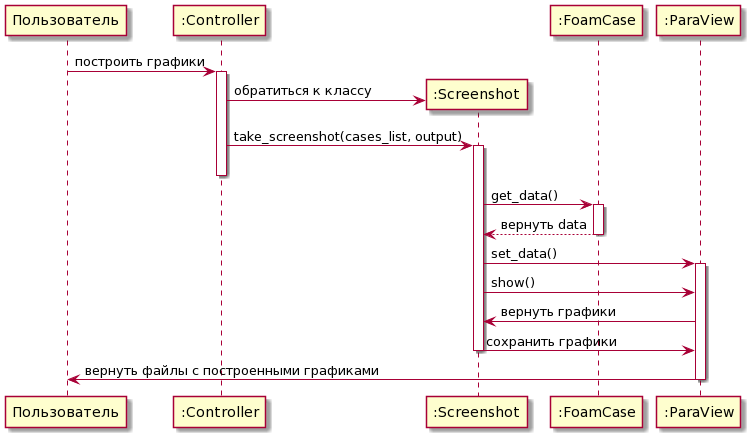
\includegraphics[width=1.1 \linewidth]{sequenceDiagram_graphs}}
\caption{Диаграмма последовательностей для прецедента <<Построение графиков примера>>}
\label{fig9}
\end{figure}

Код генерации диаграммы последовательностей для прецедента <<Сохранение примера в базу данных>>:
\begin{Verbatim}[numbers=left,xleftmargin=5mm,fontsize=\small]
@startuml
Пользователь -> ":Controller" : сохранить пример
":Controller" -> ":MongoDaoFactory" : get_dao() 
activate ":MongoDaoFactory"
":MongoDaoFactory" -> ":Controller" : инстанцировать и вернуть экземпляр MongoFoamCaseDAO
deactivate ":MongoDaoFactory"
":Controller" -> ":MongoFoamCaseDAO": create_or_update(case)
activate ":MongoFoamCaseDAO"
":MongoFoamCaseDAO" -> ":Controller": успех
deactivate ":MongoFoamCaseDAO"
":Controller" -> Пользователь: запись завершена
deactivate ":Controller"
@enduml
\end{Verbatim}

В соответствии с рисунком ~\ref{fig10} представлена диаграмма последовательностей для прецедента <<Сохранение примера в базу данных>>.
Как видно из диаграммы обращение к базе данных происходит по средствам соответствующего DAO-класса, экземпляр которого в свою очередь создается методом класса MongoDaoFactory.
\begin{figure}[H]
\centerline{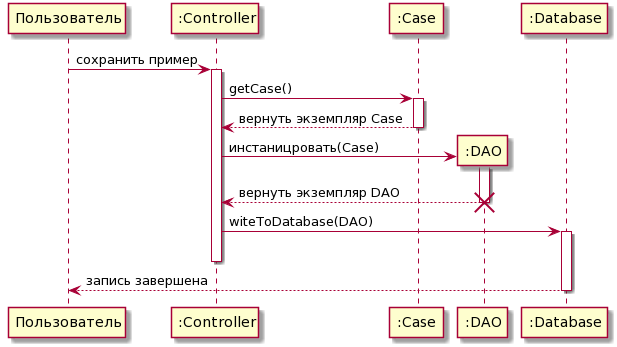
\includegraphics[width=1.1 \linewidth]{sequenceDiagram_saveToDB}}
\caption{Диаграмма последовательностей для прецедента <<Сохранение примера в базу данных>>}
\label{fig10}
\end{figure}

В соответствии с рисунком ~\ref{fig11} рассмотрена диаграмма последовательностей для прецедента <<Добавление источника данных>>. 

На данной диаграмме хорошо видно как взаимодействуют классы, меняя общее состояние программы хранящиеся в классе SharedState. Также на этой диаграмме хорошо видно как класс Controller инкапсулирует основную логику работы программы.

\begin{figure}[H]
	\centerline{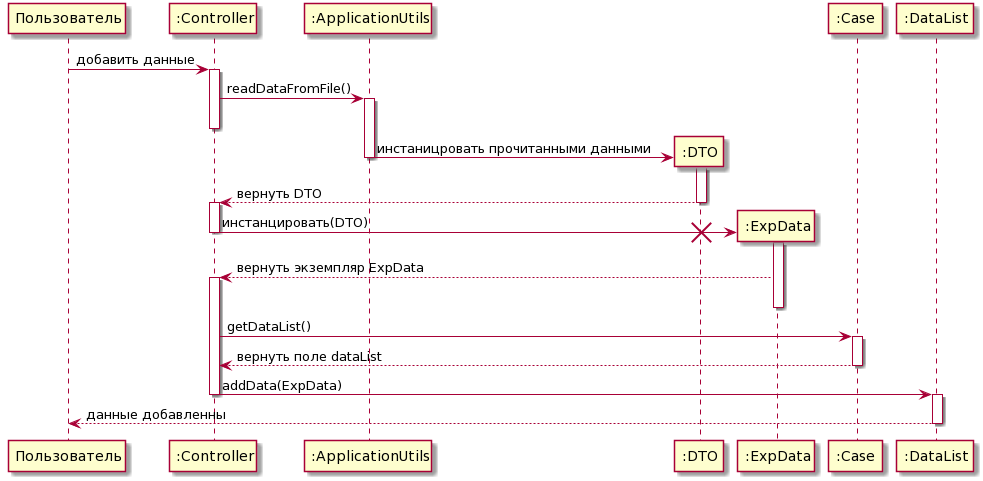
\includegraphics[width=1.1 \linewidth]{sequenceDiagram_addData}}
	\caption{Диаграмма последовательностей для прецедента <<Добавление источника данных>>}
	\label{fig11}
\end{figure}

 Код генерации:
\begin{Verbatim}[numbers=left,xleftmargin=5mm,fontsize=\small]
@startuml
Пользователь -> ":Controller" : добавить данные
activate ":Controller"
":Controller" -> ":CasesDir" : инстанцирует casesdir
":CasesDir" -> ":Controller" : возвращает casesdir
":Controller" -> ":FoamCase" : инстанцирует foamcase(casedir)
activate ":FoamCase"
":FoamCase" -> ":Controller" : возвращает foamcase
deactivate ":FoamCase"
":Controller" -> ":SharedState" : case_list().append(foamcase)
activate ":SharedState"
":SharedState" -> ":Controller" : успех
deactivate ":SharedState"
":Controller" -> Пользователь : add_item(foamcase.name)
deactivate ":FoamCase"
deactivate ":CasesDir"
":Controller" -> ":SharedState" : get_selected_case() 
activate ":SharedState"
":SharedState" -> ":Controller" : возвращает выбранный foamcase
deactivate ":SharedState"
":Controller" -> ":CameraProps" : инстанцирует camprop
activate ":CameraProps"
":CameraProps" -> ":Controller" : возвращает экземпляр camprop
deactivate ":CameraProps"
":Controller" -> ":SharedState" : foamcase.cam_prop_list.append(camprop)
activate ":SharedState"
":SharedState" -> ":Controller" : успех
deactivate ":SharedState"
":Controller" -> Пользователь : add_item(foamcase.name)
deactivate ":Controller"
@enduml
\end{Verbatim}

\chapter{Выбор средств разработки}
Для хранения данных был выбран NoSQL подход. Этот выбор обусловлен теми преимуществами, которые предоставляют СУБД этого вида, а именно:
\begin{itemize}
\item Не требуется иметь строгую схему данных.
\item Линейная масштабируемость.
\end{itemize}

В качестве базы данных приложения была выбрана документоориентированная СУБД MongoDB, как одна из наиболее известных СУБД это вида. Рассмотрим данную базу данных и сам подход NoSQL.


\section{NoSQL}
NoSQL (с английского not only SQL, что означает не только SQL). Это обозначение широкого класса различных систем управления базами данных, появившихся в период с конца 2000-х -- начала 2010-х годов и существенно отличающихся от традиционных реляционных СУБД с доступом к данным средствами языка SQL. Применяется к системам, в которых делается попытка решить проблемы масштабируемости и доступности за счёт полного или частичного отказа от требований атомарности и согласованности данных \cite{nosqlFauler}. 

Существует несколько видов NoSQL СУБД:
\begin{itemize}
	
	\item База данных <<ключ-значение>>. Это наиболее простой вариант хранилища данных, использующий ключ для доступа к значению в рамках большой хэш-таблицы \cite{nosqlAws}. Такие СУБД применяются для хранения изображений, создания специализированных файловых систем, в качестве кэшей для объектов, а также в масштабируемых Big Data системах, включая игровые и рекламные приложения, а также проекты интернета вещей (Internet of Things, IoT). Наиболее известными представителями нереляционных СУБД типа key-value считаются Oracle NoSQL Database, Berkeley DB, MemcacheDB, Redis, Riak, Amazon DynamoDB, которые поддерживают высокую разделяемость, обеспечивая беспрецедентное горизонтальное масштабирование, недостижимое при использовании других типов БД \cite{nosqlTp}.
	
	
	\item Документоориентированные СУБД. В ней находятся данные представленные парами ключ-значение, которые сжимаются в виде полуструктурированного документа из тегированных элементов, подобно JSON, XML, BSON и другим подобным форматам \cite{nosqlAws}. Такая модель хорошо подходит для каталогов, пользовательские профилей и систем управления контентом, где каждый документ уникален и изменяется со временем \cite{nosqlTp}.  Поэтому чаще всего документные NoSQL-СУБД используются в CMS-системах, издательском деле и документальном поиске. Примеры документно-ориентированных нереляционных баз данных -- это CouchDB, Couchbase, MongoDB, eXist, Berkeley DB XML  \cite{nosqlWiki}.
	\item Колоночная база данных. Хранит информацию в виде разреженной матрицы, строки и столбцы которой используются как ключи. В мире Big Data к колоночным хранилищам относятся базы типа «семейство столбцов» (Column Family). В таких системах сами значения хранятся в столбцах (колонках), представленных в отдельных файлах. Благодаря такой модели данных можно хранить большое количество атрибутов в сжатом виде, что ускоряет выполнение запросов к базе, особенно операции поиска и агрегации данных. Наличие временных меток (timestamp) позволяет использовать такие СУБД для организации счётчиков, регистрации и обработки событий, связанных со временем: системы биржевой аналитики, IoT/IIoT-приложения, систему управления содержимым и так далее Самой известной колоночной базой данных является Google Big Table, а также основанные на ней Apache HBase и Cassandra. Также к этому типу относятся менее популярные ScyllaDB, Apache Accumulo и Hypertable.
	\item Графовая база данных. Такие хранилища представляют собой сетевую базу, которая использует узлы и рёбра для отображения и хранения данных \cite{nosqlTp}. Поскольку рёбра графа являются хранимыми, его обход не требует дополнительных вычислений (как соединение в SQL). При этом для нахождения начальной вершины обхода необходимы индексы. Обычно графовые СУБД поддерживают ACID-требования и специализированные языки запросов (Gremlin, Cypher, SPARQL, GraphQL и так далее). Такие СУБД используются в задачах, ориентированных на связи: социальные сети, выявление мошенничества, маршруты общественного транспорта, дорожные карты, сетевые топологии. Примеры графовых баз: InfoGrid, Neo4j, Amazon Neptune, OrientDB, AllegroGraph, Blazegraph, InfiniteGraph, FlockDB, Titan, ArangoDB.	
\end{itemize}

Обратимся еще раз к документоориентированной СУБД. Она включает в себя кодировку документа, хранит метаданные, связанные с хранимой информацией, что даёт возможность делать запросы на основе это информации. 
Учитывая сказанное выше и также то, что такие базы данных работают без схемы данных, делает добавление полей в JSON-документы достаточно простой задачей. 

Таким образом, имеется возможность сразу хранить некий аналог объектно-ориентированной модели, что упрощает написание соответствующих классов в программе.

\section{MongoDB} 
В качестве документоориентированной СУБД была использована MongoDB, ввиду ее популярности и простоте освоения.

В рейтинге СУБД MongoDB прочно удерживается среди десяти лучших баз данных, занимая в нем пятую позицию \cite{dbrating}.


MongoDB -- это база данных документов с открытым исходным кодом, построенная на горизонтально-масштабируемой архитектуре. Каждая строка в базе данных MongoDB представляет собой документ, описанный на языке форматирования JSON.
В ниже для примера представлен простой документ JSON с описанием контактной информации \cite{nosqlMongo}.
\begin{Verbatim}[numbers=left,xleftmargin=5mm,fontsize=\small]
{
	"name" :  "Carlos Smith",
	"title" : "Product Manager",
	"location" : "New York, NY",
	"twitter" : "@MongoDB",
	"facebook" : "@MongoDB"
}
\end{Verbatim}

JSON эффективен по многим причинам:
\begin{itemize}
	\item Это естественная форма хранения данных.
	\item Легко воспринимается людьми.
	\item Структурированная и неструктурированная информация может храниться в одном документе.
    \item Благодаря JSON, документы могут иметь неограниченную вложенность друг в друга.
    \item JSON имеет гибкую и динамическую схему, поэтому добавление или удаление полей из документа не представляет каких-либо сложностей. Возможно хранить, например, частично завершенные документы.
\end{itemize}

Также важно отметить, что структура данных находится под контролем разработчика. Это в свою очередь предоставляет возможность корректировать и переформатировать базу данных по мере развития приложения без помощи администрирования базы данных. При необходимости MongoDB может координировать и контролировать изменения в структуре документов. Поля в документе играют роль столбцов в базе данных SQL, и, как столбцы, их можно индексировать для повышения производительности поиска.

MongoDB имеет хороший пользовательский web-интерфейс, что также является плюсом.

Из недостатков следует отметить ложащуюся на разработчика ответственность за формализацию базы данных. Недостаточный контроль может привести к путанице и лишним издержкам на больших проектах.

\section{Python}
Выбор языка программирования должен быть обусловлен возможностью интеграции с выбранной базой данных, а также обеспечивать доступ к Paraview API. В этой связи, будет рассмотрен язык программирования Python как наиболее подходящий кандидат.

Высокоуровневый язык программирования Python является языком общего назначения с динамической строгой типизацией и автоматическим управлением памятью, ориентированный на повышение производительности разработчика, читаемости кода и его качества, а также на обеспечение переносимости написанных на нём программ. Язык является полностью объектно-ориентированным -- всё является объектами \cite{PythonYogesh}. 
Характерное отличие языка -- выделение блоков кода пробельными символами или табуляцией. Синтаксис ядра языка минималистичен, за счёт чего на практике редко возникает необходимость обращаться к документации \cite{PythonLutz}. Python -- интерпретируемый мультипарадигмальный язык программирования, который используется для различных задач \cite{PythonYogesh}. Недостатками языка являются зачастую более низкая скорость работы и более высокое потребление памяти написанных на нём программ по сравнению с аналогичным кодом, написанным на компилируемых языках, таких как Си или C++ \cite{PythonLutz}. 

Тем не менее, Python будет легко использовать при дальнейшем расширении программы. Например, для добавления веб-интерфейса приложения можно будет использовать Django и flask. Или при что-то более легковесное, например FastAPI и React.

У приложения Paraview имеется API для двух языков: Python и C++. Это сразу ограничивает выбор языка разработки. Python более современный, комфортный и гибкий, часто выступает как более удобный интерфейс для C++ библиотек. Также Python имеет интеграцию с MongoDB через библиотеку PyMongo


В качестве языка программирования для написания работы был выбран Python, так как он достаточно гибкий и удобный, а также имеет интеграцию с ParaView через библиотеку ParaView Python API и с MongoDB через библиотеку PyMongo.

Немаловажная деталь -- это выбор среды разработки. К этому следует также подходить внимательно, так как верно выбранная среда разработки сильно сокращает время написания, отладки и тестирования программы. Остановимся PyCharm Community Edition от компании JetBrains.
Среда разработки обеспечивает:
\begin{itemize}
\item Помощь в написании кода и анализ с автозавершением кода, подсветкой синтаксиса и ошибок, быстрыми исправлениями.
\item Навигация по проекту и коду: специализированные представления проекта, представления структуры файлов и быстрое переключение между файлами, классами, методами и способами использования.
\item Рефакторинг Python: включает переименование, извлечение метода, введение переменной, введение константы, подтягивание, нажатие и другие,
\item Встроенный отладчик Python.
\item Интегрированное модульное тестирование с построчным покрытием кода.
\item Интеграция контроля версий: единый пользовательский интерфейс для Mercurial, Git, Subversion, Perforce и CVS со списками изменений и слиянием.
\end{itemize}

 Выбор обусловлен популярностью и удобством программного продукта и тем, что средства отладки и автозаполнения кода предоставляются из коробки. Это дает возможность не тратить время на установку и налаживание работы. Также в PyCharm присутствует интеграция виртуальным окружением Anaconda, которое сильно упрощает процесс подключения ParaView Python API.
Скриншот окна программы представлен в соответствии с рисунком ~\ref{fig12}.
\begin{figure}[H]
	\centerline{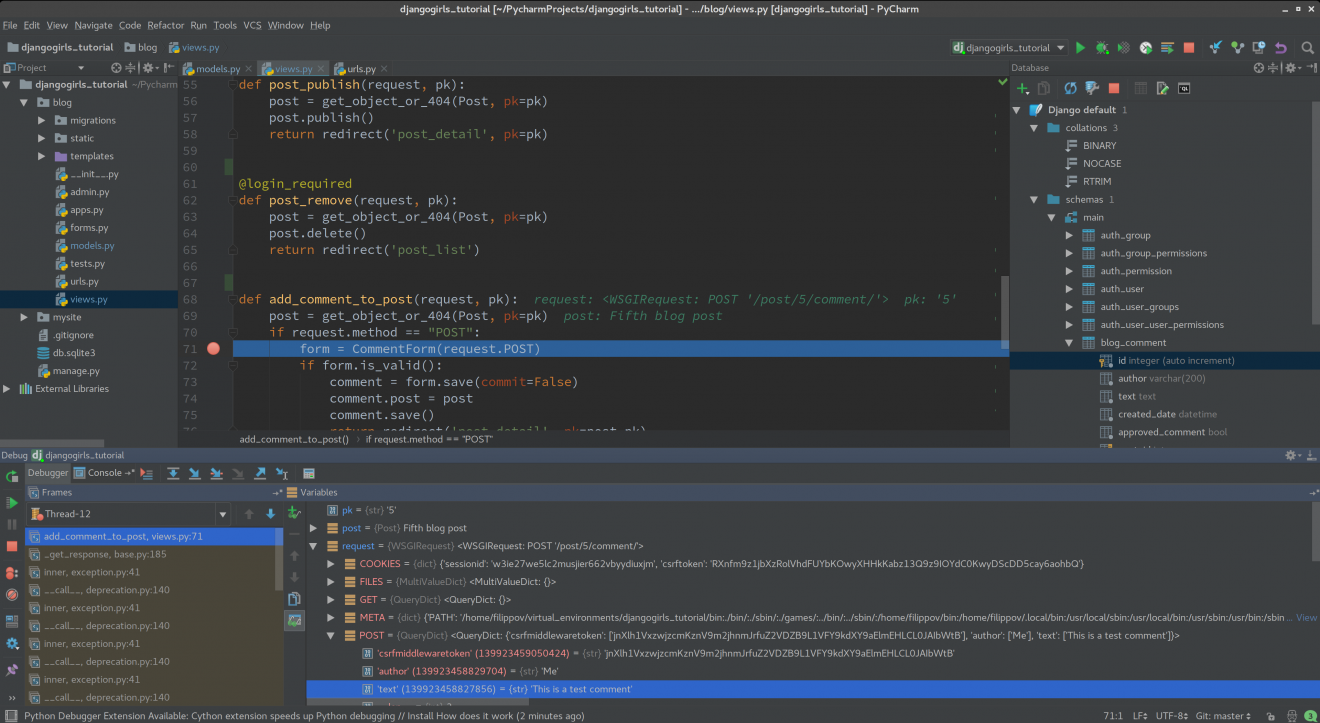
\includegraphics[scale=0.35]{pycharm}}
	\caption{Рабочее окно программы PyCharm}
	\label{fig12}
\end{figure}

 Таким образом, перечисленные выше преимущества объясняют выбор конкретно этой среды разработки. 

\section{Обзор средств разработки графического интерфейса пользователя}
Также необходимо выбрать фреймворк для разработки графического интерфейса пользователя приложения. Принимая во внимание, что мы разрабатываем на Python и, учитывая, потенциальную расширяемость программы.  

\subsection{Kivy}
Kivy -- это бесплатный фреймворк Python с открытым исходным кодом для разработки мобильных приложений и другого программного обеспечения для  широкого назначения с естественным пользовательским интерфейсом. Он распространяется в соответствии с условиями лицензии MIT, что дает право использовать библиотеку бесплатно в личных и коммерческих целях. Kivy может работать на Android, iOS, Linux, macOS и Windows \cite{kivy}. 

\begin{figure}[H]
	\centerline{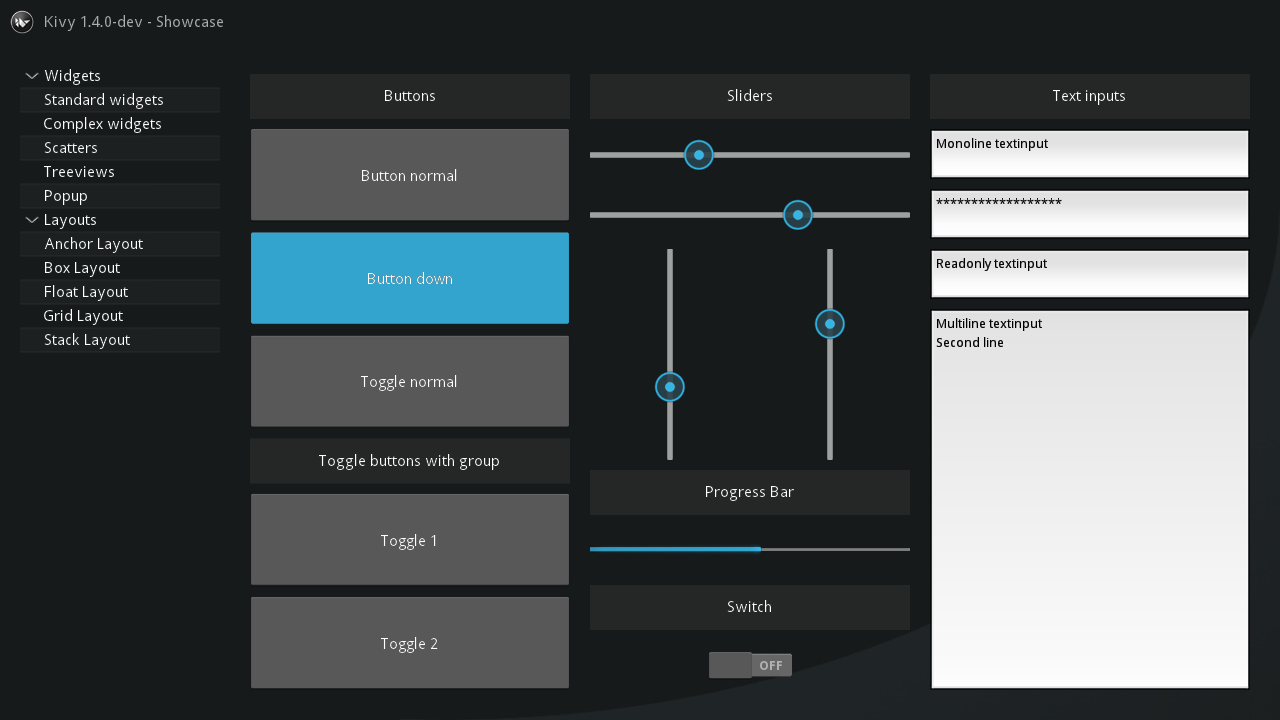
\includegraphics[width=1.1 \linewidth]{kivy}}
	\caption{Приложение Kivy}
	\label{fig13}
\end{figure}

Фреймворк содержит все элементы для создания приложения, такие как:
\begin{itemize}
\item Расширенная поддержка ввода для мыши, клавиатуры, TUIO и событий мультитач ОС.
\item Графическая библиотека, использующая только OpenGL ES 2 и основанная на Vertex Buffer Object и шейдерах.
\item Широкий выбор виджетов, поддерживающих мультитач.
\item Промежуточный язык, используемый для простой разработки пользовательских виджетов.
\end{itemize}

\subsection{TKinter}

Tkinter -- это событийно-ориентированная кросс-платформенная графическая библиотека. Она достаточно широко распространена в мире GNU/Linux и других UNIX‐подобных систем, портирована также и на Microsoft Windows. Входит в стандартную библиотеку Python и является свободным программным обеспечением.

Преимущества:
\begin{itemize}
	\item	 Краткость. Программы Python, использующие Tkinter, могут быть весьма короткими. Например, для многих используемых для создания виджетов параметров, значениям по умолчанию заданы разумные значения, что в комбинации с Python дает весьма компактный код.
	
	\item Кросс-платформенный. Tk предоставляет виджеты для Windows, Mac и большинства реализаций Unix. При это существуюет зависимость от платформы, но небольшая.
	
	\item Ядро хорошо разработано и стабильно
	
	\item Расширяемость. Существует множество расширений Tk.

\end{itemize}

Недостатки Tkinter -- скорость. Большинство вызовов Tkinter форматируются как Tcl-команда и интерпретируются c помощью Tcl. Отсюда фактические и выполняются вызовы Tkinter. Таким образом происходит последовательный вызов двух интерпретируемых языков \cite{pythonRob}.

\subsection{wxPython}
wxPython - это кроссплатформенный набор инструментов с графическим интерфейсом для языка программирования Python. Он позволяет программистам Python просто и легко создавать программы с графическим пользовательским интерфейсом. Он реализован в виде набора модулей расширения Python, которые обертывают компоненты графического интерфейса популярной кроссплатформенной библиотеки wxWidgets, написанной на C++ \cite{wxpython}.

Подобно Python и wxWidgets, wxPython является открытым исходным кодом. Также он является кроссплатформенным инструментарием. В настоящее время поддерживаемыми платформами являются Microsoft Windows, Mac OS X и macOS, а также Linux или другие unix-подобные системы с библиотеками GTK2 или GTK3.

Присутствует официальная документация, но не хватает сторонних источников и примеров использования библиотеки.

\begin{figure}[H]
	\centerline{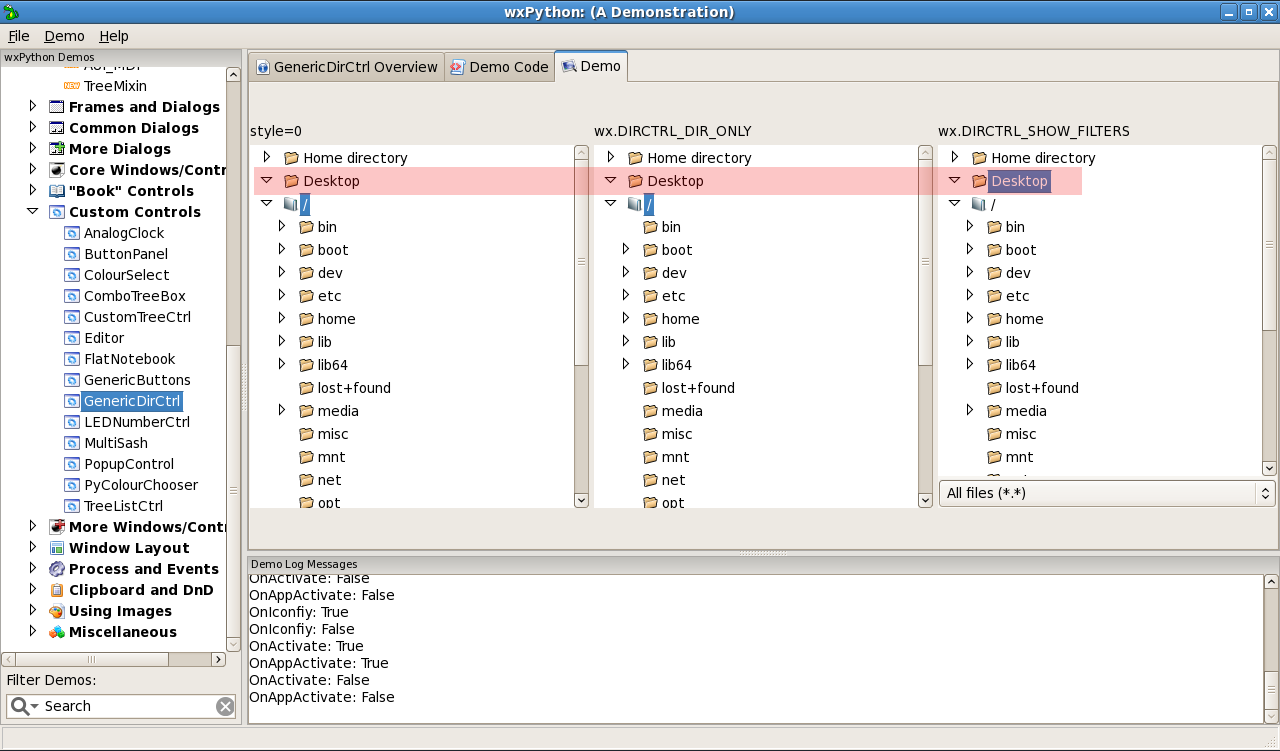
\includegraphics[width=1 \linewidth]{wxpython}}
	\caption{Пример использующей wxPython программы}
	\label{figwxpython}
\end{figure}

\subsection{PyQt/PySide}
PyQt — набор расширений (биндингов) графического фреймворка Qt для языка программирования Python, выполненный в виде расширения Python.

PyQt работает на всех платформах, поддерживаемых Qt: Linux и другие UNIX-подобные ОС, Mac OS X и Windows. Существует 2 версии: PyQt5, поддерживающий Qt 5, и PyQt4, поддерживающий Qt 4. PyQt распространяется под лицензиями GPL (2 и 3 версии) и коммерческой \cite{pyqt}. 

PyQt также включает в себя Qt Designer (Qt Creator) — дизайнер графического интерфейса пользователя. Программа pyuic генерирует Python код из файлов, созданных в Qt Designer. Это делает PyQt очень полезным инструментом для быстрого прототипирования. Кроме того, можно добавлять новые графические элементы управления, написанные на Python, в Qt Designer. 

Однако, для PyQt существуют ограничения связанные с лицензией GPL, поэтому был разработан PySide. PySide -- привязка языка Python к инструментарию Qt, совместимая на уровне API с PyQt. В отличие от PyQt, PySide доступна для свободного использования как в открытых, так и закрытых, в частности, коммерческих проектах, поскольку лицензирована по LGPL \cite{pyside}. 

Все представленные библиотеки имеют примерно одинаковые преимущества, но стоит выбирать наиболее зрелые и популярные. Это даст возможность в случаи необходимости легко найти решение проблем, возникающих в процессе разработки приложения. PySide кажется хорошим вариантом.

\begin{figure}[H]
	\centerline{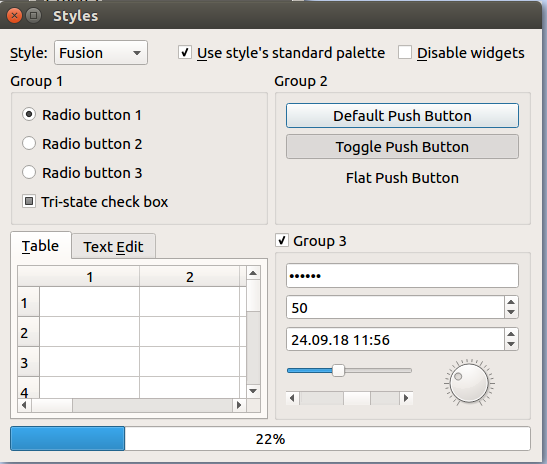
\includegraphics[scale=0.7]{pyqtscreenshot}}
	\caption{Приложение, написанное с помощью PySide}
	\label{fig14}
\end{figure}

Преимущества PySide с точки зрения выбора фреймворка:
\begin{itemize}
	\item Стабильность.
	\item Подробнейшая документация.
	\item Обилие дополнительной информации на различных форумах и сайтах.
\end{itemize}

Недостатки:
\begin{itemize}
	\item Сложность в освоении из-за большого размера.
	\item Не вся документация доступна для языка Python.
\end{itemize}

Но эти недостатки нивелируются. В частности, первый из них не имеет значения, если есть некий опыт работы и общее понимание принципов устройства фреймворка. А второй недостаток, также преодолевается опытом,подобием синтаксиса в целом и большим количеством сторонней информации в сети интернет.

Таким образом, предпочтение было отдано PySide. 

\chapter{Разработка информационной системы}
В соответствии с рисунком ~\ref{fig15} представлен скриншот разработанной программы. 
\begin{figure}[H]
	\centerline{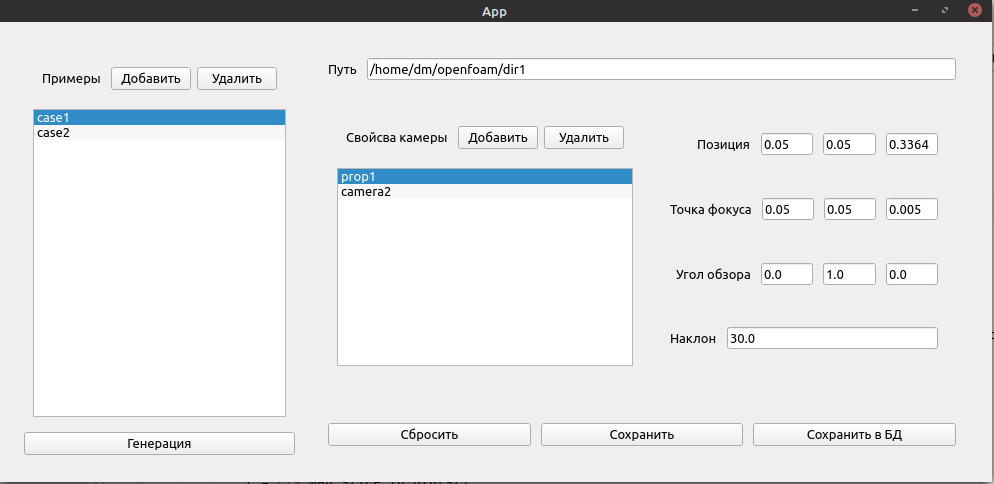
\includegraphics[scale=0.5]{app}}
	\caption{Разработанное приложение}
	\label{fig15}
\end{figure}

Разработка была начата с модуля model. В нем содержаться классы модели данных: FoamCase, CameraProps, Point, CaseDir. Затем были разработаны соответствующие им DTO-классы (Data Trasfer Object). После этого был написан класс Mapper для отображения DTO в model и обратно. Затем нужно было приступить к разработке DAO слоя и схемы базы данных. 

На самом деле, так как была использована документоориентированная СУБД MongoDB, то необходимость в проектировки схемы базы данных отпала, однако, все же нужно было создать коллекции и получить доступ к хранилищу. В соответствии с рисунком ~\ref{figdb} показан web-интерфейс созданного в результате экземпляра базы данных MongoDB. 

Также для объектной модели требовалось добавить поля \_id во все классы и DTO объекты соответственно. Поля \_id нужно было инициализировать, используя класс ObjectId из библиотеки PyMongo. С этим были связаны некоторые трудности, так как класс Mapper также пришлось переписывать, учитывая нововведения.


\begin{figure}[H]
	\centerline{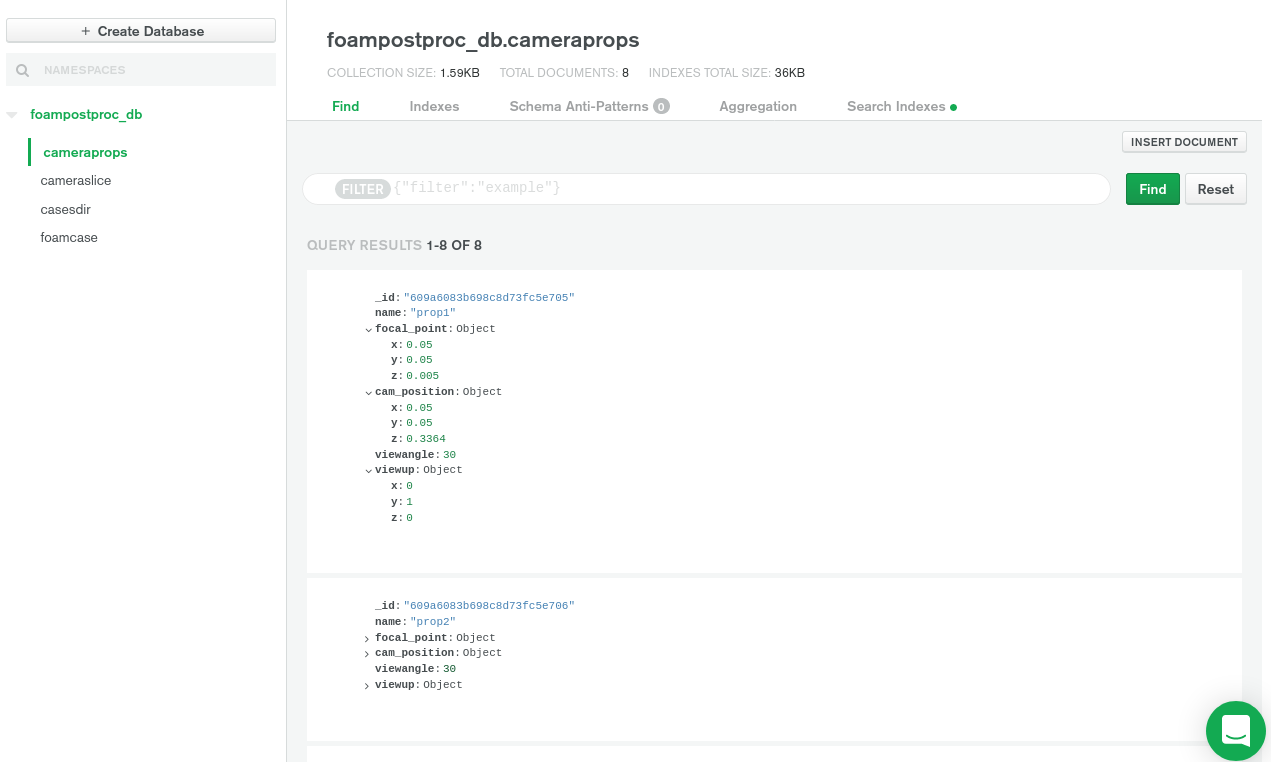
\includegraphics[scale=0.4]{db}}
	\caption{Web-интерфейс экземпляра базы данных MongoDB}
	\label{figdb}
\end{figure}

Параллельно с этим возникали трудности с работой в ParaView Python API. Данная библиотека плохо документирована. На официальном сайте есть краткие пояснения назначения методов, но совершенно отсутствует описание классов и их полей, также на официальном сайте отсутствует описание процесса работы с библиотекой и какие-либо полезные примеры.

Большое время заняло подключение ParaView Python API к виртуальному окружению Python. Следует отметить, что результата удалось достичь только используя окружение Anaconda. В окружении Anaconda, в свою очередь, возникли проблемы с установкой соответствующих пакетов, что в последствии привело к трудностям с запуском PySide6. 

Более того, после успешного подключения библиотеки возникали трудности с подсказками методов, что очень сильно тормозило работу (принимая во внимание отсутствие полезной документации).

Тем не менее, получения тестовых графиков от ParaView Python API, был разработан DAO-слой, который отвечает за доступ к базе данных. После чего был сделан графический интерфейс пользователя. И оставшееся время было потрачено на написание класса Controller. Он отвечает за обработку событий вызванных графическим интерфейсом пользователя и объединяет элементы программы, а именно: 
\begin{itemize}
	\item Модель
	\item Графический интерфейс пользователя
	\item Логику отвечающую за создание и редактирование примеров
	\item Логику генерацию графиков
\end{itemize}

В завершении работы был добавлен класс Config, который обращается к соответствующему файлу, куда были вынесены параметры программы, например логин и пароль от базы данных и передает их классам для работы.

Исходный код программы приведен в соотвествии с приложением А.

\chapter{Пример анализа экспериментальных данных}

Как было сказано ранее, при обработке экспериментальных данных, когда проводится серия экспериментов, в которых входные данные незначительно изменяются, часто порождается большой объем результатов, подлежащих анализу или, иными словами, постобработке. Для анализа таких данных необходимо проводить однотипные манипуляции. 

Например, рассматривается движение вязкой жидкости в каверне. Такое движение описывают уравнения Навье-Стокcа. Уравнения Навье-Стокса -- система дифференциальных уравнений в частных производных, описывающая движение вязкой ньютоновской жидкости. Уравнения Навье -- Стокса являются одними из важнейших в гидродинамике и применяются в математическом моделировании многих природных явлений и технических задач. 

Геометрия течения показана в соответствии с рисунком \ref{fig20} в которой все границы квадрата являются твердыми стенками длинной 0.1 м. Верхняя стенка перемещается в x-направлении со скоростью 1 м/с, в то время как другие 3 неподвижны.

\begin{figure}[H]
	\centerline{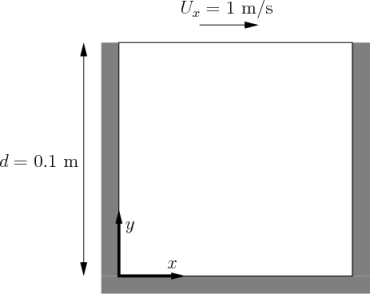
\includegraphics[scale=1.4]{cavity}}
	\caption{Геометрия расчетной области задачи}
	\label{fig20}
\end{figure}


Пусть для уравнениях Навье-Стокса в случае несжимаемых жидкостей потребовалось построить графики скорости для последовательно увеличивающейся кинематической вязкости. 

Задав положение камеры и директорию с расчетами или загрузив эти данные из базы данных запустим генерацию графиков и оценим результаты. 

Графики были построены для коэффициентов вязкости соответственно от 0.01 до 0.18 с шагом 3, либо 2. Для краткости приведем три из них: первый, затем из середины и последний график.


\begin{figure}[H]
	\centerline{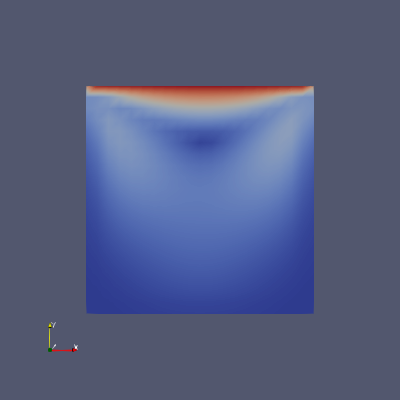
\includegraphics[scale=1.0]{res1}}
	\caption{График с коэффициентов вязкости 0.01}
	\label{fig16}
\end{figure}

В соответствии с рисунком ~\ref{fig16}, в соответствии с рисунком ~\ref{fig17} и в соответствии с рисунком ~\ref{fig18} видно, что пока рос коэффициент вязкости графики практически не менялись, но ближе к концу заметен резкий всплеск.

\begin{figure}[H]
	\centerline{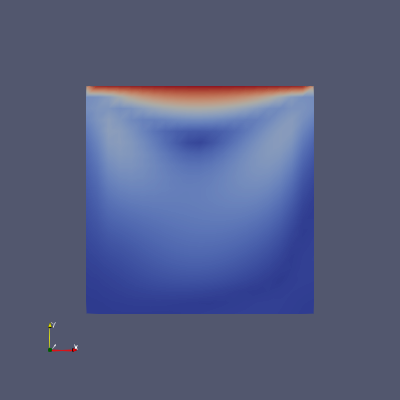
\includegraphics[scale=1.0]{res2}}
	\caption{График с коэффициентов вязкости 0.09}
	\label{fig17}
\end{figure}

\begin{figure}[H]
	\centerline{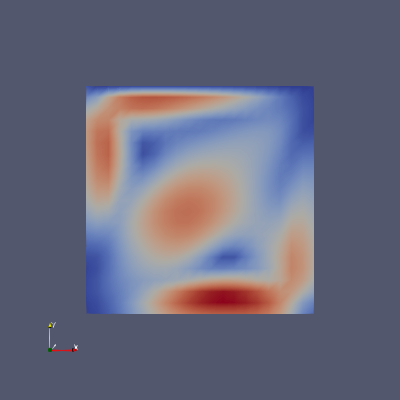
\includegraphics[scale=1.0]{res3}}
	\caption{График с коэффициентов вязкости 0.18}
	\label{fig18}
\end{figure}

\begin{figure}[H]
	\centerline{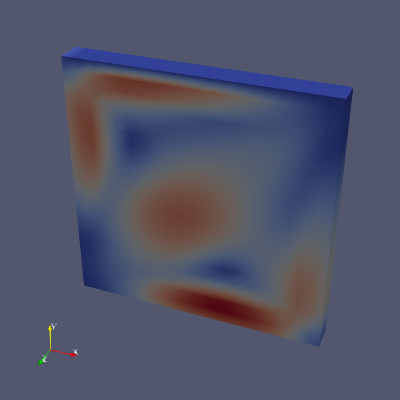
\includegraphics[scale=1.0]{res3-dc}}
	\caption{График с коэффициентов вязкости 0.18 с другого ракурса}
	\label{fig19}
\end{figure}

\conclusions
При обработке экспериментальных данных и расчетов, полученных в результате математического моделирования физических процессов когда проводится серия экспериментов, в которых входные данные незначительно изменяются порождается большой объем результатов, подлежащих постобработке.

Как было указано во введении, целью данной магистерской работы является проектирование и разработка информационной системы, автоматизирующей рутинные операции анализа экспериментальных данных для CAD/CAE систем. 
Конкретизируя цель, были поставлены следующие задачи:
\begin{itemize}
	\item Кратко рассмотреть платформу для численного моделирования OpenFOAM и пакет для визуализации ParaView. 
	
	Благодаря решению этой задачи понятие CAD/CAE приложение было уточнено до конкретного решения -- пакет программ OpenFOAM и инструмент постобработки ParaView, таким образом неявно был очерчен контекст разработки приложения.
	\item Рассмотреть существующие решения по данной тематике.
	
	 При решении этой задачи были проанализированные существующие на данный момент программы, предоставляющие похожий функционал автоматизации моделирования. Были приведены их преимущества и недостатки, а также было дано некоторое обоснование актуальности разрабатываемого приложения.
	\item Спроектировать информационную систему и создать UML-диаграммы для ее описания. 
	
	В рамках этой задачи была проведена основная работа по проектированию приложения, очерчен его контур и структура связей. Также были подробно рассмотрены основные классы программы, приведены примеры кода построения UML-диаграмм и результат их генерации.
	\item Провести обзор средств разработки. 
	
	Здесь были рассмотрены средства разработки, последовательно обоснован выбор определенных инструментов. В некоторых случаях приведено сравнения с аналогичными по функционалу библиотеками и фреймворками.
	
	\item Разработать помогающую в анализе экспериментальных данных информационную систему.
	
	Решая эту задачу, был подробно описан процесс разработки и возникшие в ходе нее проблемы.
\end{itemize}

Дополнительно был добавлен раздел с примером анализа экспериментальных данных при помощи разработанного приложения.

Таким образом, в данной работе был кратко рассмотрен пакет программ для численного моделирования OpenFOAM, приложение для постпроцессинга ParaView. Было выполнено проектирование, в частности построены UML-диаграммы прецедентов, классов, последовательностей. Также были рассмотрены существующие на данный момент решения постобработки экспериментальных данных и выбраны средства разработки. 

Было разработано приложение, которое выполняет одну из подзадач разработки и анализа экспериментальных данных, в частности программа строит графики указанных расчетов по заданным параметрам и хранит данные, используемые для построения в БД, используя NoSQL подход. Программа позволяет не тратить время при постобработке ряда слабо отличающихся друг от друга геометрией и условиями данных, генерируя графики группами сразу для всех расчетов. Этим она отличается и выделяется на фоне рассмотренных решений.  

Сама разработка носит итеративный процесс, поэтому трудно судить о полноте выполненных задач в плане написания кода. Однако, можно с некоторой долей уверенности сказать, что минимально жизнеспособный продукт был создан, но еще много деталей требуют внимания и дальнейшего развития.

Таким образом, задачи данной работы были выполнены и, следовательно, поставленная цель была достигнута. 


% Оформляем библиографию в соответствии с ГОСТ 7.0.5
\bibliographystyle{ugost2008}
% если хотим включить все источники из библиографии даже не имеющие ссылки из текта
% \nocite{*}
% файл с библиографией
% \bibliography{biblio.bib}

\begin{thebibliography}{9}

\bibitem{OpenfoamWiki} 
   Статья OpenFOAM [Электронный ресурс] : (на 08 апреля 2021 года) // Официальный веб-сайт Wikipedia [Электронный ресурс] : [сайт]. - URL: https://ru.wikipedia.org/wiki/OpenFOAM (дата обращения 08.04.2021). - Загл с экрана - Яз. рус.
   
\bibitem{OpenfoamUserGuide} 
   Страница User guide [Электронный ресурс] : (на 08 апреля 2021 года) // Официальный веб-сайт OpenFOAM [Электронный ресурс] : [сайт]. - URL: https://cfd.direct/openfoam/user-guide (дата обращения 08.04.2021). - Загл с экрана - Яз. англ.
   
\bibitem{ParaviewAbout} 
   Страница About [Электронный ресурс] : (на 08 апреля 2021 года) // Официальный веб-сайт ParaView [Электронный ресурс] : [сайт]. - URL: https://www.paraview.org/overview (дата обращения 08.04.2021). - Загл с экрана - Яз. англ.
   
\bibitem{ParaviewWiki} 
   Статья ParaView [Электронный ресурс] : (на 09 апреля 2021 года) // Официальный веб-сайт Wikipedia [Электронный ресурс] : [сайт]. - URL: https://ru.wikipedia.org/wiki/ParaView (дата обращения 09.04.2021). - Загл с экрана - Яз. рус.
   


\bibitem{ParaviewAndPython} 
   Страница ParaView and Python [Электронный ресурс] : (на 10 апреля 2021 года) // Официальный веб-сайт ParaView [Электронный ресурс] : [сайт]. - URL: https://www.paraview.org/Wiki/ParaView\_and\_Python (дата обращения 10.04.2021). - Загл с экрана - Яз. англ.
  
\bibitem{Helyx} 
   Продукт Helyx OS [Электронный ресурс] : (на 29 марта 2021 года) // Официальный веб-сайт Helyx [Электронный ресурс] : [сайт]. - URL: https://engys.com/products/helyx-os (дата обращения 29.03.2021). - Загл с экрана - Яз. англ.
      
\bibitem{Ansa} 
   Продукт ANSA [Электронный ресурс] : (на 11 апреля 2021 года) // Официальный веб-сайт компании Beta [Электронный ресурс] : [сайт]. - URL: http://www.beta-cae.gr/ansa.html (дата обращения 11.04.2021). - Загл с экрана - Яз. англ.
   
\bibitem{CastNet} 
   Продукт CastNet [Электронный ресурс] : (на 11 апреля 2021 года) // Официальный веб-сайт компании DHCAE Tools [Электронный ресурс] : [сайт]. - URL: http://www.dhcae-tools.com/CastNet.html (дата обращения 11.04.2021). - Загл с экрана - Яз. англ.  

\bibitem{umlDistilled}
  Фаулер, М. UML. Основы, 3-е издание/ М. Фаулер -- Спб: Символ-Плюс, 2004. - 192 с.
  
\bibitem{oop}
  Гамма, Э. Приемы объектно-ориентированного проектирования/ Э. Гамма, Р. Хелм, Р. Джонсон, Д. Влиссидес -- Спб: Питер, 2019. - 368 с.
  
\bibitem{pattern-factory} 
  Паттерны проектирования. Фабрика [Электронный ресурс] : (на 19 апреля 2021 года) // Веб-сайт refactoring guru [Электронный ресурс] : [сайт]. - URL: https://refactoring.guru/ru/design-patterns/factory-method (дата обращения 19.04.2021). - Загл с экрана - Яз. рус.

\bibitem{pattern-proxy} 
Паттерны проектирования. Заместитель [Электронный ресурс] : (на 19 апреля 2021 года) // Веб-сайт refactoring guru [Электронный ресурс] : [сайт]. - URL: https://refactoring.guru/ru/design-patterns/proxy (дата обращения 19.04.2021). - Загл с экрана - Яз. рус.  

\bibitem{umlApplying}
  Ларман, К. Применение UML 2.0 и шаблонов проектирования. Практическое руководство. 3-е издание/ К. Ларман -- М: И.Д. Вильямс, 2013. - 736 с.
  
\bibitem{nosqlFauler}
     Фаулер М. NoSQL. Методология разработки нереляционных баз данных / М. Фаулер, П. Садаладж -- Диалектика-Вильямс, 2021. - 192 с.
     
\bibitem{nosqlAws} 
Обзор NoSQL [Электронный ресурс] : (на 19 апреля 2021 года) // Веб-сайт Amazon Web Services [Электронный ресурс] : [сайт]. - URL: https://aws.amazon.com/ru/nosql/ (дата обращения 19.04.2021). - Загл с экрана - Яз. рус.

\bibitem{dbrating} 
DB-Engines Ranking [Электронный ресурс] : (на 19 апреля 2021 года) // Веб-сайт DB Engines [Электронный ресурс] : [сайт]. - URL: https://db-engines.com/en/ranking (дата обращения 19.04.2021). - Загл с экрана - Яз. англ.



\bibitem{nosqlTp} 
Разбираемся в типах NoSQL СУБД [Электронный ресурс] : (на 19 апреля 2021 года) // Веб-сайт Tproger [Электронный ресурс] : [сайт]. - URL: https://tproger.ru/translations/types-of-nosql-db/ (дата обращения 19.04.2021). - Загл с экрана - Яз. рус.

\bibitem{nosqlWiki} 
NoSQL СУБД [Электронный ресурс] : (на 20 апреля 2021 года) // Веб-сайт wikipedia [Электронный ресурс] : [сайт]. - https://ru.wikipedia.org/wiki/NoSQL (дата обращения 20.04.2021). - Загл с экрана - Яз. рус.


\bibitem{nosqlMongo} 
MongoDB [Электронный ресурс] : (на 23 апреля 2021 года) // Веб-сайт mongodb [Электронный ресурс] : [сайт]. - https://www.mongodb.com/why-use-mongodb (дата обращения 23.04.2021). - Загл с экрана - Яз. англ.

\bibitem{PythonYogesh}
Yogesh R., Python: Simple though an Important Programming language [Текст]  / R. Yogesh // International Research Journal of Engineering and Technology (IRJET). – 2019. - том 06, номер 2. – С. 1856—1858.

\bibitem{PythonLutz}
Лутц, М. Программирование на Python, том 1 / М. Лутц -- СПб: Символ-Плюс, 2011. - 992 с.

\bibitem{IDEComp}
Сравнение интегрированных сред разработки [Электронный ресурс] : (на 24 апреля 2021 года) // Веб-сайт wikipedia [Электронный ресурс] : [сайт]. - https://en.wikipedia.org/wiki/Comparison\_of\_integrated\_development\_\\environments\#Python (дата обращения 24.04.2021). - Загл с экрана - Яз. англ.

\bibitem{kivy}
Страница о нас [Электронный ресурс] : (на 30 апреля 2021 года) // Веб-сайт фреймворка Kivy [Электронный ресурс] : [сайт]. - https://kivy.org/\#aboutus (дата обращения 30.04.2021). - Загл с экрана - Яз. англ.

\bibitem{pyqt}
PyQt. Введение [Электронный ресурс] : (на 30 апреля 2021 года) // Веб-сайт Riverbank Computing [Электронный ресурс] : [сайт]. - https://riverbankcomputing.com/software/pyqt/intro (дата обращения 30.04.2021). - Загл с экрана - Яз. англ.

\bibitem{pyside}
Qt for Python [Электронный ресурс] : (на 30 апреля 2021 года) // Веб-сайт Wiki Qt [Электронный ресурс] : [сайт]. - https://wiki.qt.io/Qt\_for\_Python/ru (дата обращения 30.04.2021). - Загл с экрана - Яз. рус.

\bibitem{pythonRob}
Robinson A. Python Programming On Win32 / A. Robinson, M. Hammond -- O'Reilly Media, 2000. - 674 с.

\bibitem{wxpython}
Overview of wxPython [Электронный ресурс] : (на 30 апреля 2021 года) // Веб-сайт wxPython [Электронный ресурс] : [сайт]. - https://www.wxpython.org/pages/overview/ (дата обращения 30.04.2021). - Загл с экрана - Яз. англ.

\end{thebibliography}


\Appendix
\chapter{Исходный код программы}
\section{foampostproc.core.screenshot.taker.py}
Модуль используется для генерации графиков.
\lstinputlisting{code/taker.py}
\section{foampostproc.core.controller.py}
Модуль содержит класс Controller, который инкапсулирует основную логику работы с моделью.
\lstinputlisting{code/controller.py}
\section{foampostproc.core.model.py}
Модуль состоит из классов, описывающих структуру данных приложения.
\lstinputlisting{code/model.py}
\section{foampostproc.core.view.py}
В данному модуле содержится код графического интерфейса пользователя.
\lstinputlisting{code/view.py}
\section{foampostproc.dao.dao.py}
Модуль, хранящий классы DAO-слоя программы.
\lstinputlisting{code/dao.py}
\section{foampostproc.dao.daofactory.py}
Данный модуль хранит класс-фабрику для классов DAO-слоя.
\lstinputlisting{code/daofactory.py}
\section{foampostproc.dto.dto.py}
Этот модуль хранит DTO-классы.
\lstinputlisting{code/dto.py}
\section{foampostproc.dto.modelmapper.py}
Модуль содержит функции, которые отображают DTO-объекты в соответствующие им классы модели и наоборот.
\lstinputlisting{code/modelmapper.py}
\section{foampostproc.config.py}
Модуль, содержащий код для работы с файлом конфигурации программы.
\lstinputlisting{code/config.py}
\section{foampostproc.main.py}
Модуль, содержащий точку входа в программу и производящий начальные настройки приложения.
\lstinputlisting{code/main.py}
\section{foampostproc.utils.py}
Модуль, содержащий разные полезные функции например чтение JSON файлов или константы указывающие путь к корневой директории приложения. Также здесь находится общее состояние программы.

\lstinputlisting{code/utils.py}


\end{document}
